\documentclass{assignment}
\begin{document}

\begin{titlepage}
    \begin{center}
        % University Logo
        
\includegraphics[width=4cm]{assets/logo.png} \\[1cm]

        \vfill 
        {\Large \textbf{İstanbul Üniversitesi}} \\[0.5cm]

        % Faculty / Department
        {\large Edebiyat Fakültesi \\ Tarih Bölümü} \\[1.5cm]

        {\huge \textbf{MÜZE UYGULAMALARI II}} \\[0.5cm]
        {\Large Öğretim üyesi: Dr. Burcu Kutlu Dilbaz} \\[1cm]

        \vfill 
        % Author Information
        {\large Hazırlayan:} \\[0.2cm]
        {\Large Yiğit Çağrı Akkaya} \\[0.2cm]
        {\large Ö\"{g}renci Numarası: 0302220014} \\[0.2cm]
        \vfill
        {\large \today}
    \end{center}
\end{titlepage}

\tableofcontents
\newpage

\indent\indent Bu rapor, İstanbul Üniversitesi Tarih Bölümü Dr. Öğr. Üyesi Burcu Kutlu Dilbaz tarafından verilen Müze Uygulamaları II(TARH3071) dersinde anlatılanlar, incelenen eserler, ders notları ve öğrencinin kendi araştırmları baz alınarak hazırlanmıştır.
\section{Birinci Hafta - Türk İslam Eserleri Müzesi}
\indent\indent Türk ve İslam Eserleri Müzesi’ndeki bu ilk dersimizde, müzenin halı sergileri salonunda, Hocamız Dr. Öğr. Üyesi Burcu Kutlu Dilbaz tarafından müzelerin tarihi ve önemi, müzelere giriş, Osmanlı Devleti’nde müzenin kuruluşu ve Türkiye'de müzelerin tarihi nedir ve nasıl gelişmiştir konuları anlatıldı.
\subsection{Koleksiyonculuktan Müzeye}
\indent\indent Müzeciliğin kökenleri bulmak için, tarih boyunca insanların oluşturduğu koleksiyonlara bakmalıyız. Genellikle varlıklı ve zengin insanlar, tarih boyunca birtakım objeleri toplayarak koleksiyon haline getirmişlerdir. En erken koleksiyon izlerine Antik Mısır'da rastlıyoruz. Tutankhamon'un mezarı açıldığında, içinden 5000 parçaya yakın kişisel eşyaları ve müceverhat ortaya çıkmıştır. Buna tam anlamıyla bir koleksiyon diyemesek de, erken çağlardan itibaren insanların mücevher gibi değerli eşyaları topladığına dair bir ipucu veriyor bize. Yine Hıristiyanlığın erken dönemlerinden itibaren kiliselerin ikona, kutsal emanet(relic) ve el yazmaları topladığını biliyoruz.\newline
\indent Koleksiyonculuk, 16.yüzyıl itibariyle daha popüler bir hale gelmeye başladı. Koleksiyon sahiplerinin başında hükümdarlar geliyordu. Antik Mısır'da olduğu mücverehat yine en önemli kolleksiyon eşyasıydı. Bunun yanında kitaplar, el yazmaları, Rönesans ile birlikte resim, heykel gibi sanat eserleri koleksiyon eşyalarının başında geliyordu. Hükümdarların yanı sıra bazı zenginler ve önemli devlet adamları da koleksiyonerler arasında yerlerini almaya başladı. Toplanan bu eşyalar, evlerin ve sarayların içinde sergi için özel olarak tasarlanmış odalarda, vitrin ile muhafaza edilerek gelen misafirlere sergilenmeye başlandı. Bu odalar, günümüz müzelerin ilk adımı oldu.\newline
\indent Koleksiyon boyutları büyüdükçe, bunları halka sergilemek için özel bina oluşturma fikri ortaya çıktı. Bu bağlamda 1677 yılında Oxford üniversitesi'nde yapımına başlanan Ashmolean Müzesi, 1683 yılında açıldı. Sir Hans Sloane'nın koleksiyonu, 1753'teki ölümünden sonra British Museum oluşturularak burada sergilenmeye başlandı. Fransız kraliyet koleksiyonları ise 1793'te monarşinin feshi ile kamulaştırıldı ve Louvre Sarayı'nda(bugün Louvre Müzesi) sergilenmeye başlandı. İtalya'da ise Anna Maria Luisa 'de Medici, kişisel sanat koleksiyonunu Floransa'da sergilenmesi şartıyla 1737 yılında Uffizi Galerisi'ne bağışladı. Rusya'da ise II.Katerina, kendi özel koleksiyonu için 1764 yılında Hermitage Müzesi'ni kurdu. Hermitage ancak 1852 yılında halka açıldı. İspanya'da kraliyet koleksiyonunu sergilemek için 1819 yılında Prado Müzesi(\textit{Museo Del Prado}) kuruldu.
\subsection{Osmanlı Devleti'nde İlk Müzecilik Girişimleri}
\indent\indent Rönesans ile Avrupa'da Yunan ve Roma uygarlıklarına olan ilgi arttı. Bunun sonucunda pek çok gezgin antik Yunan ve Roma şehirlerini ziyaret etmeye başlamıştır. 18.yüzyılın ikinci yarısından sonra bu ilgi Mısır'ı da içine almaya başladı. Bu ilginin sebebini, Avrupalılar'ın Osmanlı toprakları üzerinde hak sahibi olma kaygısından dolayı olduğu ileri sürülmüştür.\cite{shaw} Bunun sonucunda 19.yüzyılın başında Osmanlı topraklarında yabancılar tarafından kazılar yapılmaya başlandı. Bu dönemde Osmanlı Devleti'nde eski eser kavramı tam olarak yoktu. Eski eserlerin hukuki durumunu fıkıh belirlemiştir. Hangi tür arazide bulunursa bulunsun, sahibi belli olmayan eşyalar için aşağıdaki kurallar uygulanır.\cite{mumcu_1}
\begin{enumerate}[label=\alph*)]
    \item üstü kelime-i şehadet ya da İslam için tanınmış başka bir işaret ile süslü ise bu eşyalar lukata(bulunutu mal) hükmündedir. Lukata hükümlerine göre, eşyayı bulan, malın sahibinin ortaya çıkması için durumu beyan eder. Sonuç alınazmsa bulan kişinin ekonomik durumuna bakılır. Yoksul ise kendisi alır, zengin ise ya fakirlere ya da Beytülmal'a alır.
    \item üzerinde İslamdan başka dinlere ait işaretler ya da İslam olmayan hükümdarların adları kazınmış eşyaların beşte biri Beytülmal'a alınır. Geriye kalanı, arazi padişah tarafından kime tahsis edildiyse ona ya da mirasçılarına verilir. Eğer arazi kimseye tahsis edilmemişse ve miri de değilse, eşyanın geri kalanı bulana verili. Bulan kişi Osmanlı Devleti vatandaşı değilse bu haktan faydalanamaz. Yalnızca padişah izni ile define arayanlar, kendisine verilen hisseyi alabilir.
    \item Bulunan eşyanın kategorisi belirlenemiyorsa, (b) bendindeki hükümler uygulanır.
\end{enumerate}
\indent\indent Buradan anlaşılıyor ki, kazı sonucu bulunan eşyalara el koymak oldukça kolaydır. Bu kayıtsızlığın sebebini belki de Osmanlı Devleti'nin eski eser tanımında aramak gerekir. Fıkhın belirlediği maddelerden de anlaşılacağı gibi, Osmanlı Devleti Türk-İslam kültüründe değerli olan eşyaları eser olarak görüyordu. Büyük bir imparatorluk olduğu için, kendi içinden çıkan değerlere önem veriyordu. Bu noktada antik Yunan ve Roma medeneyitlerine ait kalıntılara önem verdiğini söyleyemeyiz. Bundan dolayıdır ki, 19.yüzyılda padişahtan kazı izni almak oldukça kolaydı. Bu izinler, 1840'larda Maarif Nezareti'nin yetkisine verilmiştir.\cite{dilbaz_1}\newline
\indent Osmanlı Devleti'nde ilk müze girişimi, eski eserlerin \textit{Mecma-ı Eslah-ı Atik}(Eski Silahlar Koleksiyonu) ve \textit{Mecma-ı Âsâr-ı Atîka}(Eski Eserler Koleksiyonu) adı altında, o dönem silah deposu olarak kullanılan  Aya İrini'de  Tophane Müşiri Fethi Ahmet Paşa tarafından toplanması ortaya çıkmıştır.\cite{degirmenci} Bu girişime tam olarak bir müze demek doğru olmayacaktır; çünkü eserlerin toplanma amacı sergilemesinden çok koruma altına alınmasıydı. Fethi Ahmet Paşa, 1858'deki ölümüne kadar eserlerin Aya İrini'de toplanması görevini yürüttü. Fethi Ahmet Paşa'nın ölümünden 11 yıl sonra Aya İrini, Maarif Nazırı Saffet Paşa tarafından \textit{Müze-i Humay\^{u}n} adı altında ziyarete açıldı. Maarif Nazırı Saffet Paşa'nın diğer bir önemli icraatı ise, vilayetlere gönderdiği yazılar ile ortaya çıkan eski eserlerin Müze-i Humay\^{u}n'a gönderlimesini buyurmasıydı. Bunun sonucunda, kısa bir süre sonra Aya İrini toplanan eski eserler için yetersiz kalmaya başladı. Yeni müze binası olarak Topkapı Sarayı'ndaki Çinili Köşk tayin edildi. Eserlerin Çinili Köşk'e taşınması 1881 yılında tamamlanmış ve yeni Müze-i Humay\^{u}n törenle açılmıştır. Burası, bugünkü İstanbul Arkeoloji Müzesi'nin çekirdeğini oluşturacaktır.
\indent Müze-i Humayûn'un ilk müdürü olarak Mekteb-i Sultânî tarih öğretmenlerinden  Edward Goold(1868-1871) atandı. Müzenin ikinci müdürü, bu görevi yaklaşık bir yıl kadar sürdürecek olan Pio Francesco Carlo Terenzio'dur. Terenzio'dan boşalan koltuğa 1872 yılında Philipp Anton Dethier oturmuş ve bu görevi 1881 yılına kadar sürdürmştür.\cite{saatci}
\subsection{1869 Asar-ı Atika Nizamnamesi}
\indent\indent 1869 yılına kadar Osmanlı Devleti'nde eski eserlerin durumunu fıkıh dışında belirleyen bir kanun ya da nizamname bulunmamaktaydı. 1869 yılında, Sadrazam Ali Paşa'nın sadareti dönemimde eski eserlerle ilgili ilk nizamname yayınlanmıştır. Bu nizamnamenin giriş kısmında birtakım tespitlere ve hususlara yer verilmiş, Maarif Nezareti'nin girişimiyle kaleme alındığı belirtilip, maddelere geçilmiştir. Tespitler, hususları ve maddeler aşağıdaki gibi özetlenebilir:\cite{karaduman}
\subsubsection{Tespitler}
\begin{itemize}
    \item Eski eserlerin Osmanlı Devleti topraklarında çokça bulunması
    \item Kazılar için ruhsat verilirken çift olarak bulunan eski eserlerin bir tekinin Devlet-i Aliyye'ye verilmesi usulunun, ikili eserlerin pek nadir çıkmasından ya da ikili çıkanlarının bir eşinin saklanmasından dolayı uygulanamaması
\end{itemize}
\subsubsection{Hususlar}
\begin{itemize}
    \item Eski eserlerin kıymet ve öneminden dolayı yapılacak araştırma ve kazıların yazılı kurallara bağlanması
    \item Müzenin düzenlenerek mevcut eserlerin kayıt altına alınması, sergilenmesi ve eksiklerinin giderilmesi hususlarının Maarif Nezareti'ne bağlanması
    \item Müzenin masraflarının karşılanması için adı geçen bakanlığa ücret tahsisi
\end{itemize}
\subsubsection{Maddeler}
\begin{itemize}
    \item Eski eser kazı ve araştırması yapacak kişiler, Maarif Nezareti'nden izin almadıkça hiçbir kazı yapamayacaktır.
    \item Kazı ve araştırma izni alan kişilerin buldukları eski eserleri yurt dışına çıkaramayacaktır. İçeride talep olursa, bu eserleri Devlet-i Aliyye'ye satma hakları mevcuttur.
    \item Özel mülkte çıkan eski eserler mülk sahibinin olacaktır.
    \item Bulunan sikkeler, yurt dışına çıkarma yasağından muaftır.
    \item Eski eser araştırması izni yalnızca toprak altını kapsamaktadır.
    \item Bir devletin resmi olarak eski eser talebinde bulunması halinde, bu talebin kabul edilip yerine getirilmesi Padişah'ın özel iznine bağlıdır.
    \item Eski eser araştırma ve kazılarında uzman olan kişilere, masrafları ve ücretleri hazine tarafından karşılanmak üzere memuriyet ve resmi izin verilecektir. Bu nedenle, söz konusu kişiler ilgili nezarete başvuruda bulunacaktır.
\end{itemize}
\subsection{1874 Asar-ı Atika Nizamnamesi}
\indent\indent 1869 çıkarlan nizamname, eski eserler hukuku üzerine sadece bir başlangıç oldu. Kısa sürede bu ilk nizamnamenin yetersizliği anlaşıldığı için 1874 yılında daha detaylı bir şekilde, ikinci bir nizamname yayınlandı. 34 maddeden oluşan bu nizamnameyi şu şekilde özetleyebiliriz.\cite{mumcu_2}
\begin{itemize}
    \item İlk iki madde eski eser tanımını yapmaktadır.
    \item Sonraki dört madde esas ilkeleri açıklamaktadır. Keşfedilmemiş eski eser nerede bulunursa bulunsun, devlete aittir prensibi kabul ediliyor. İzin alarak yasal kazı yapanların buluntunun üçte birini devlete, diğer üçte birini arazi sahibine, geriye kalan üçte biri de kendisine alabileceğini belirtiyor.
    \item Sonraki maddede, önceki nizamnamede olduğu gibi, kazıları Maarif Nezareti'nin iznine bağlıyor.
    \item 8.maddeden 22.maddeye kadar kazı izni için gerekli olan şartları ve ödenmesi gereken harçları belirliyor.
    \item 23.maddede, sahipsiz alanda devlet kazı yapmak isterse başka kimseye o alanda kazı izni verilmeyeceği yasasını koyuyor.
    \item 24.maddede, devletin özel mülklerde de kazı yapabileceğini ve özel mülkte oluşan hasarı tazmin edeceğini ekliyor.
    \item Eski eser bulanların en geç 10 gün içinde mahalli devlet otoritelerine başvurması gerektiği, eğer bu yasa ihlal edilirse şahıslara devletin payının dörtte biri kadar para cezası uygulanması 25.maddede açıklanıyor.
    \item 28. maddede, buluntunun nasıl bölüştürüleceği çözülemezse, Maarif Nezareti'nin başvurulması gerektiği belirtiliyor.
    \item 31.maddeden 34.maddeye kadar, eski eserlerin satışı, ihracı ve ithalıyla ilgili yasaları ortaya koyuyor.
\end{itemize}
\subsection{Osman Hamdi Bey}
\indent\indent Modern anlamda ilk müzecilik girişimin Osman Hamdi Bey ortaya atmıştır. Osman Hamdi Bey, 10 Aralık 1842'de İstanbul'da doğmuştur. Babası İbrahim Edhem Paşa, 5 Şubat 1877 - 11 Ocak 1878 tarihleri arasında sadrazamlık görevini ifa etmiştir. Osman Hamdi Bey, 1856'da Mekteb-i Ma\^{a}rif-i Adliyye'ye kayıt olmuş ve bir sene sonra hukuk tahsili için Paris'e gitmiştir. Paris'teki eğitimi sırasında, Paris Güzel Sanatlar Yüksek Okulu'nda resim dersleri aldı. 1858'de çıktığı Viyana ve Belgrad gezilerinde, bu şehirlerdeki müzeleri ve sergileri inceleme fırsatı buldu. 12 senelik Paris macerasını, 1869'da yurda dönerek sona erdirdi. Dönemin Bağdat Valisi Mithat Paşa kendisine Vil\^{a}yet-i Um\^{u}r-ı Ecnebiyye(Vilayet Yabancı İşleri) müdürlüğünü teklif etti. Görevi kabul eden Osman Hamdi Bey Bağdat'a gitti. 1871'de İstanbul'a geri dönen Osman Hamdi Bey, 1875'te Hariciye Um\^{u}r-ı Ecnebiyye k\^{a}tibi oldu. 1877'de Beyoğlu Belediyesi Altıncı D\^{a}ire Müdürlüğüne getirildi. 1877-78 Osmanlı-Rus Savaşı sonrası memurluktan ayrılarak zamanını resme ayırdı. Müze-i Hümay\^{u}n'un müdürü Philipp Anton Dethier'in vefatı üzerine 1881'de müzenin müdürlüğüne atandı.\newline
\indent Müdürlük görevi ile Osman Hamdi Bey Osmanlı müzeciliğine yeni bir soluk getirdi. Yeni bir müze yapılması için çalışmalara başladı. Günümüzde İstanbul Arkeoloji Müzesi olan binanın ilk kısmının yapımı 1891'de tamamlandı. Bu bina kazılarda bulunan eserleri himaye etmeye yetmeyince, 1903'te ikinci kısmın, 1907'de de üçüncü kısmın inşası tamamlandı. Vefat ettiği 1910 yılına kadar müdürlük görevini sürdürdü. Müdürlüğü esnasında arkeolojik kazıları teşvik ederken, birçoğuna bizzat kendisi katıldı. Katıldığı kazılar arasında Sayda, Nemdur Dağı, Rodos, Taşoz gibi önemli kazılar da bulunmakta.\cite{dia_1}
\subsection{1884 Asar-ı Atika Nizamnamesi}
\indent\indent Osman Hamdi Bey, Müze-i Hümayûn'un müdürlüğü görevini yürütürken 1864 nizamnamesinin yetersizliğini fark etti. Girişimleri ile 1884'te üçüncü bir nizamname yayınladı. Beş bölüm ve 37 maddeden oluşan nizamname 1906 yılında gözden geçirilip tekrar yayınlandı ve 1973 yılına kadar büyük bir değişiklik geçirmeden yürürlükte kaldı.\cite{dilbaz_2} Nizamnameyi şu şekilde özetleyebiliriz:\cite{mumcu_3}
\begin{itemize}
    \item 1.maddede, 1874 nizamnamesinde olduğu gibi eski eser tanımı üzerinde durulmuş ve daha kapsamlı hale getirilmiştir.
    \item 2.maddede eski eserlerin temellük ve tassaruf hakları belirtilmiştir.
    \item 3.maddeden 6.maddeye kadar eski eserlerin korunması gerekliliği, yıkılıp kaldırılamayacağı ya da yapılar üzerinde herhangi bir değişiklik yapılamayacağı karara bağlanmıştır.
    \item 8.madde yurt dışına eser ihracını kesin ve istinisnasız olarak yasaklamıştır.
    \item 9.maddeden 27.maddeye kadara kazı için alınması gerek ruhsatnamenin şartları çizilmiştir.
    \item 33.maddeden 35.maddeye kadar eski eser hukukun uygulayacağı cezaları açıklamıştır.
    \item 36.maddede, ortaya çıkan anlaşmazlıkların adli mahkemeler tarafından çözüleceği hükme bağlanmıştır.
\end{itemize}
\section{İkinci Hafta}
\subsection{Türk İslâm Eserleri Müzesi}
\begin{wrapfigure}{r}{0.4\textwidth}
    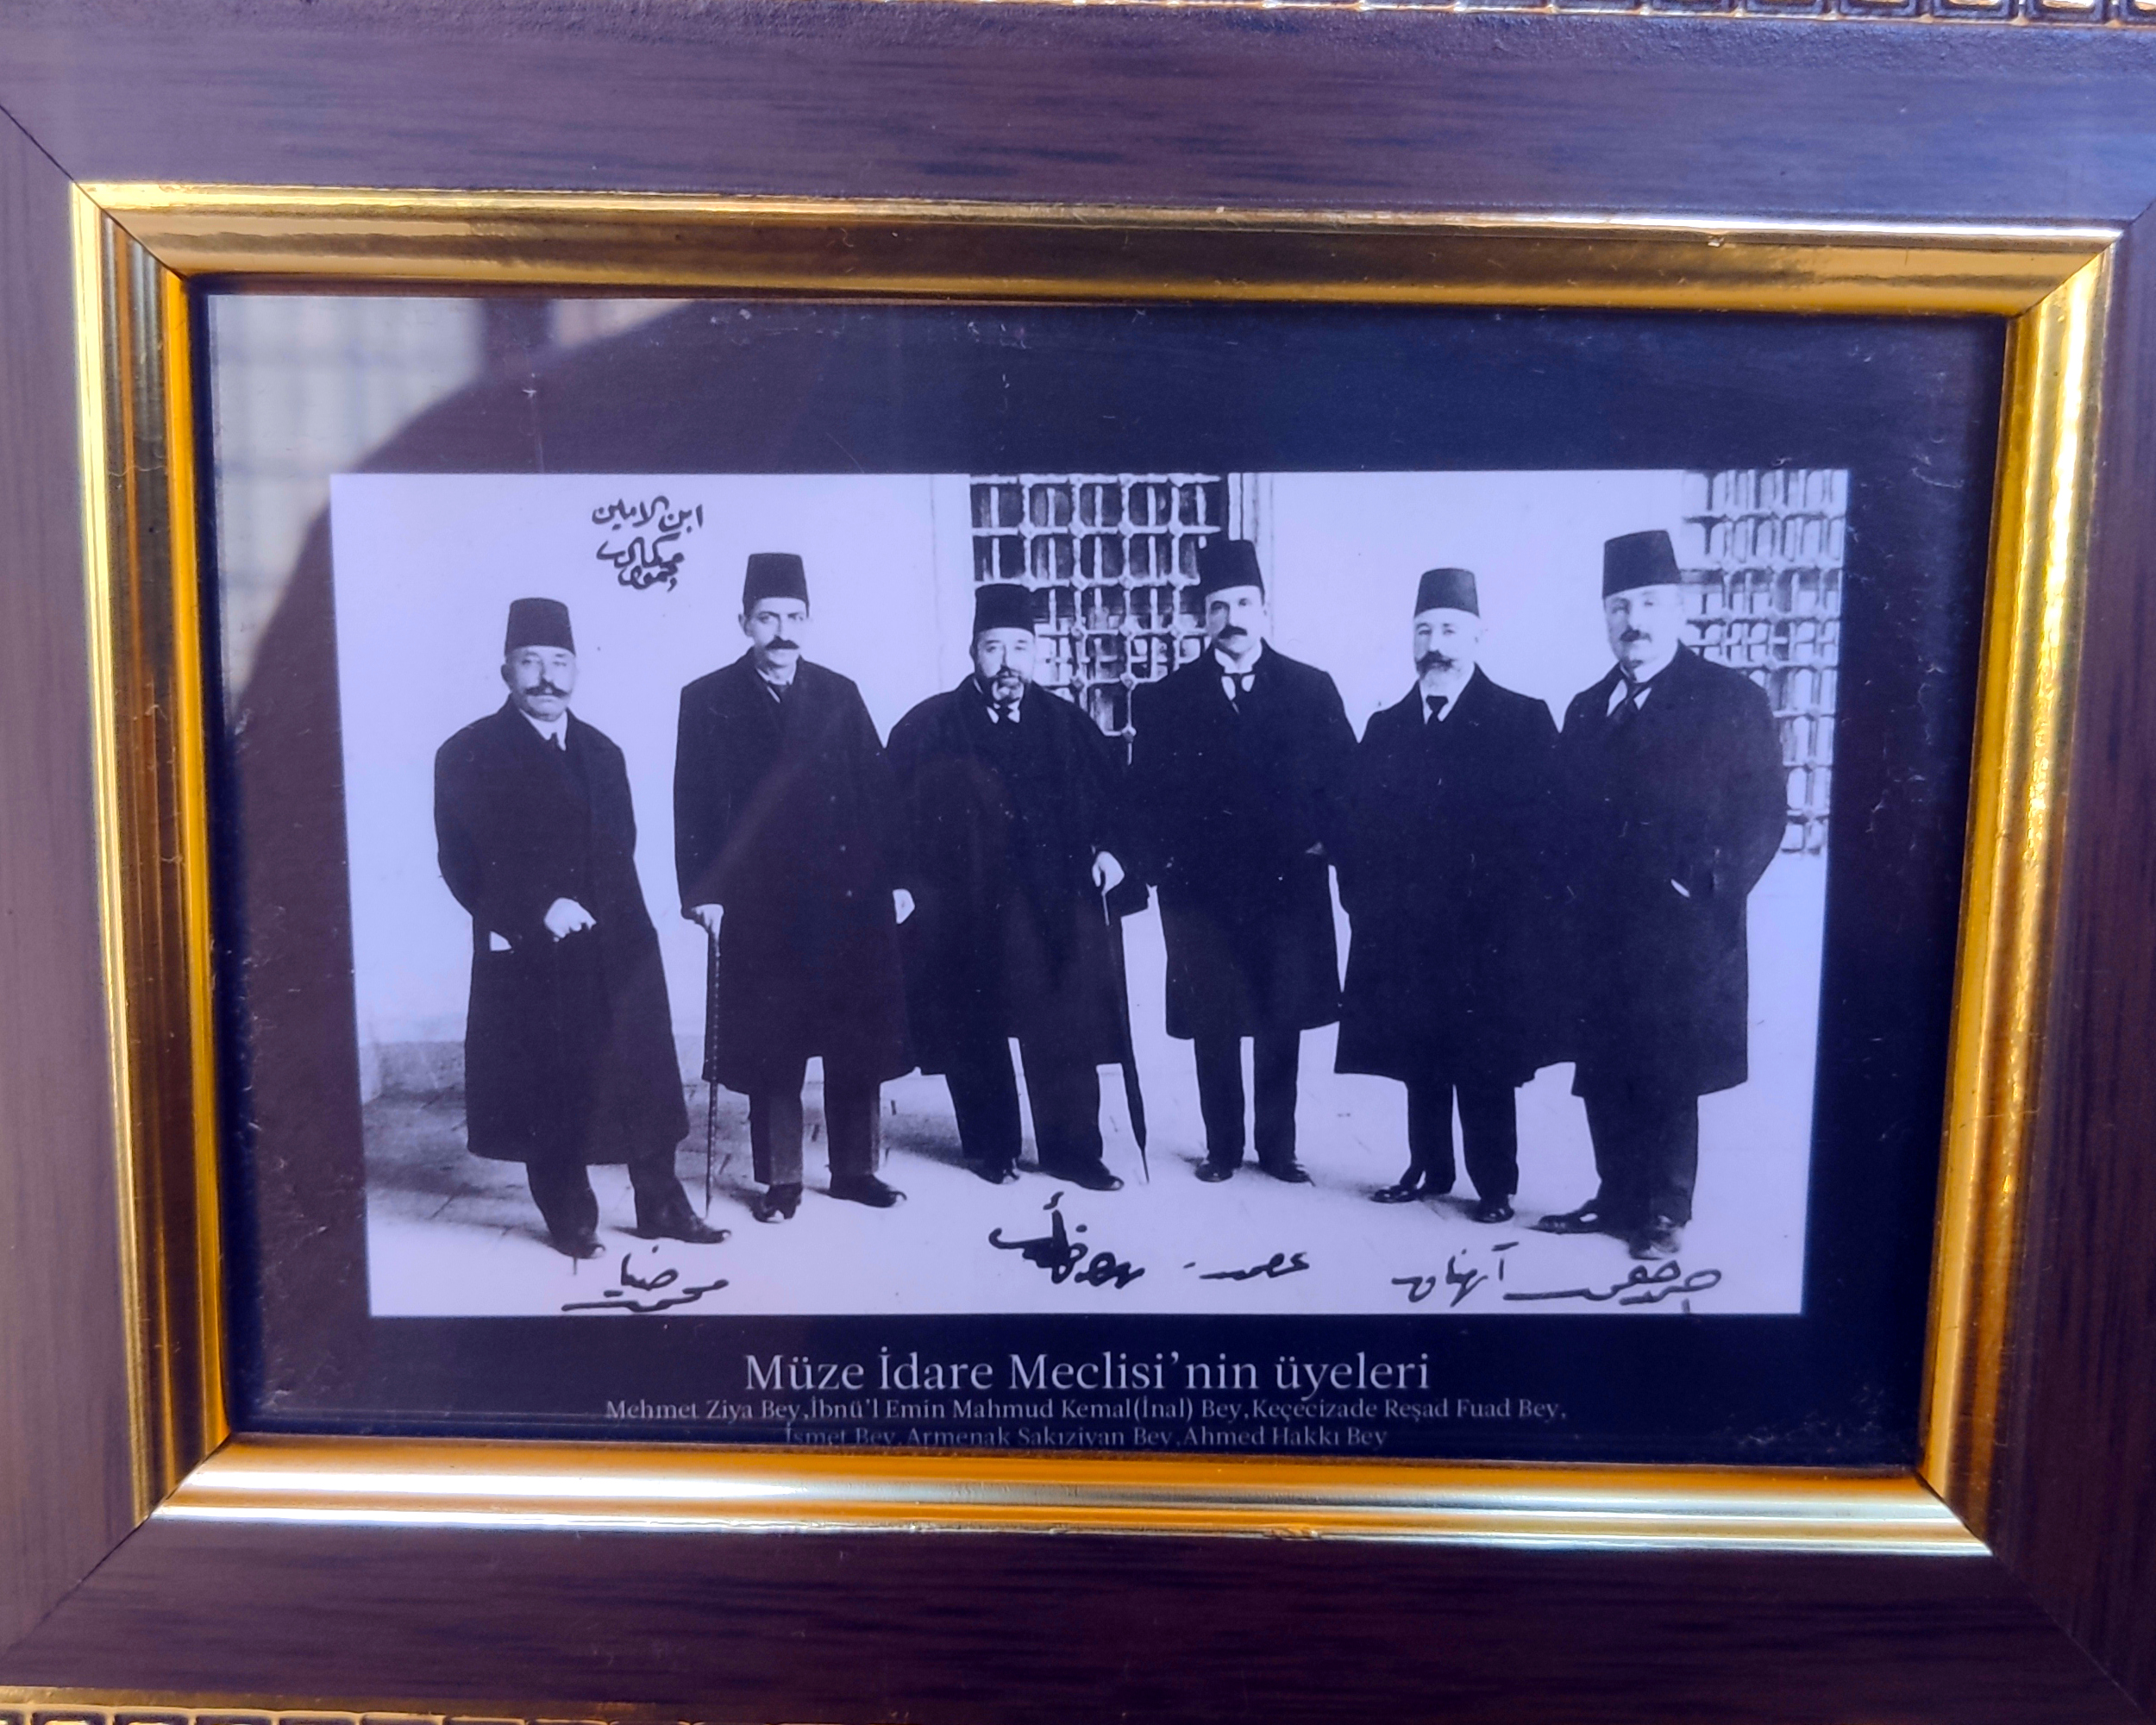
\includegraphics[width=0.4\textwidth]{assets/museum_opening.jpg}
    \caption{Müze Açılışında Bir Fotoğraf}
    \label{fig:musem_opening}
\end{wrapfigure}
\indent\indent 1908 yılından itibaren yapılan toplantılarda Sadrazamlık, Maarif Nezareti ve Müze-i Hümâyun kurumları, kıymetli eşyların yurt dışına çıkarılmasını engellemek için Hazîne-i Evkaf-ı Hümâyun İdaresi'ne bağlı bir müzede koruma altına alınmasını önermiştir. Yine aynı dönemde Sadrazam Hüseyin Hilmi Paşa'nın imzasını taşıyan tezkereler, eski eserlerin yurt dışına çıkışını engellemek için gümrüklere gönderilmiştir. Bu girişimlerin sonucunda Türk İslâm Eserleri Müzesi, 1914 yılında Evkaf-ı İslâmiyye Müzesi ismiyle Süleymaniye Camii'nin imarethanesinde kurulmuştur. Müze, 27 Nisan 1914 tarihinde, Sultan Mehmed Reşat'ın tahta çıkışının yıldönümünde açılmıştır. Açılışta Veliaht Yusuf İzettin Efendi, Sadrazam Said Halim Paşa, Şeyhülislâm Ürgüplü Hayri Efendi, Besim Ömer Paşa hazır bulunmuşlardır. Kuruluşunda Evkaf-ı Humâyun Nezareti'ne bağlı olan müze, 1924 yılında bu nezaretin kaldırılmasıyla Maarif Vekaleti'ne bağlanmıştır. Zaman içinde artan eski eserlerden dolayı, Süleymaniye Camii'nin imarethanesi yetersiz kalmış ve 1983 yılında Sultanahmet'teki İbrahim Paşa Sarayı'na taşınmıştır.\cite{dia_2}\newline
\indent İbrahim Paşa Sarayı'nın inşa tarihi bilinmemektedir. II.Bayezid döneminde yaşamış tarihçi Solakzade, At Meydanı'nda inşa edilen bir saraydan bahsetmektedir.\cite{atasoy_1} Saraya dair ilk yazılı belge 1521 yılına ait. Bu belge, mevcut sarayın tamiratını buyurmaktadır. Dört avlu, ahırlar, bir kule ve hazine binasından oluşan saray, oldukça geniş bir araziye yayılmış durumdaydı. İbrahim Paşa'nın, 1524 yılında 15gün süren düğünü yine bu sarayda yapılmıştır. İbrahim Paşa'nın 1536'daki idamı üzerinde saraya müsadere edilmiştir. Sonraki dönemlerde de saray sadrazamlara, vezirlere ve önemli devlet adamlarına tahsis edilmiştir. 1652 yılında yanan saray, 1720 civarında Nevşehirli Damat İbrahim Paşa tarafından tamir ettirilmiştir. 1741'te tekrar yanan saray bir daha onarılmamıştır.\cite{dia_3} Sarayın üçüncü avlusuna 1910 yılında Mimar Vedat Tek'in projelendirdiği Defter-i Hakani(Tapu Kadastro Müdürlüğü)(günümüzde Ayasofya Müzesi) binası yapılmıştır. Sarayın bir diğer avlusu ise 1939 yılında Adliye Sarayı'nın inşası için yıkılmıştır. 1970lerde restorasyon geçiren sarayın ikinci avlusu, 1983 yılında Türk İslâm Eserleri Müzesi'ne tahsis edilmiştir.\cite{atasoy_2}
\subsection{Müze Turu}
\indent\indent Türk İslam Müzesi, adından da anlaşılacağı gibi ağırlıklı olarak Türk ve İslam eserlerinin sergilendiği bir müze. Müze, 2012-2014 yılları arasında geçirdiği restorasyondan sonra günümüzdeki halini almıştır. Müzedeki eseler, ait oldukları dönemlere göre tasnif edilmiş olarak ayrı odalarda sergilenmektedir. Sırasıyla Abbasiler, Emeviler, Büyük Selçuklular, İlhanlılar, Timurlular, Memlûkler, Safeviler, Kaçarlar, Anadolu Selçuklular ve Osmanlılar dönemlerinden kalan eserler bulunmaktadır. Müzede öne çıkan eserler arasında el yazmaları, halı ve kilimler, Kutsal Emanetler ve şamdanlar ön plana çıkmatadır.
\subsubsection{Lahitler ve Kitabeler}
\indent\indent Müzenin girişinde iki mermer lahit bulunmakta(Şekil \ref{fig:lahit}). Bu lahitler Memlûk Halep Valisi Özdemir ve eşinini mezarları için tasalanmış olup, 1493 yılına aittir. Lahitler, ya mezarın üstüne ya da yakınına konuşlandırılan ve mezar taşı görevi taşıyan yapılardır. Yaygın kanının aksine içinde naaşı muhafaza etmemektedir.\newline
\indent Bu kısmı geçip, soldaki kapıdan devam edince karşımıza iki tane kitabe çıkıyor. Şekil \ref{fig:grave}'deki kitabe , Emeviler döneminden bir mescide aittir. Şekil \ref{fig:road_stone}'deki kitabe  ise bir mesafe taşıdır. Bu kitabe, günümüzde kilometre tabelalarının Emeviler dönemindeki eşleniğidir. Mesefa taşı kitabesi, en geç 705 yılına aittir.\newline
\begin{figure}[ht]
    \centering
    \subfigure[Özdemir ve Eşinin Lahitleri]{
        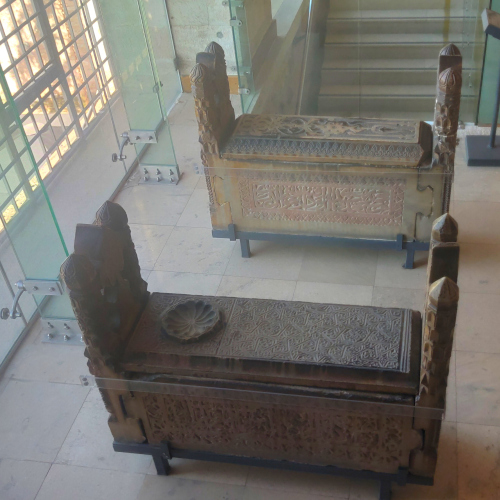
\includegraphics[height=0.3\textheight,width=0.30\linewidth]{assets/lahit.jpg}
        \label{fig:lahit}
    }
    \hfill
    \subfigure[Mescit Kitabesi]{
        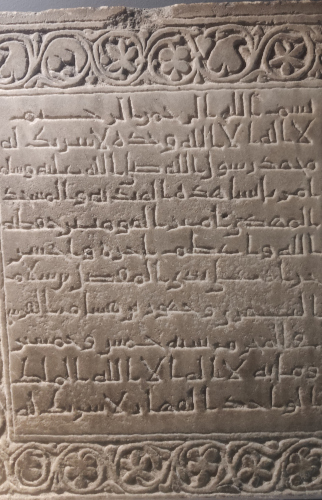
\includegraphics[height=0.3\textheight,width=0.30\linewidth]{assets/mescid.jpg}
        \label{fig:grave}
    }
    \hfill
    \subfigure[Mesafe Taşı Kitabesi]{
        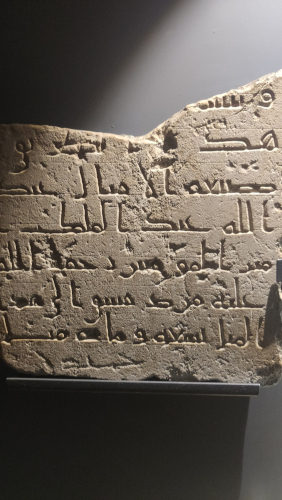
\includegraphics[height=0.3\textheight,width=0.30\linewidth]{assets/mesafe.jpg}
        \label{fig:road_stone}
    }
    \caption{Lahitler ve Kitabeler}
    \label{fig:lahits_kitabes}
\end{figure}
\subsubsection{Samarra Camii ve Rakka Seramikleri}
\begin{wrapfigure}{r}{0.4\textwidth}
    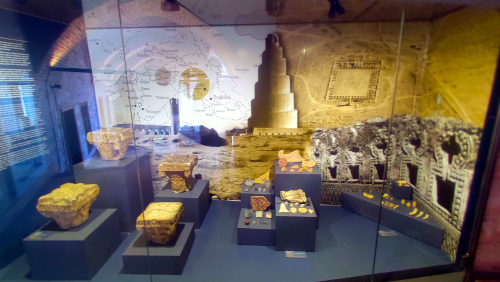
\includegraphics[width=0.4\textwidth]{assets/samarra.jpg}
    \caption{Samarra Camii}
    \label{fig:samarra}
    \vspace{10pt}
    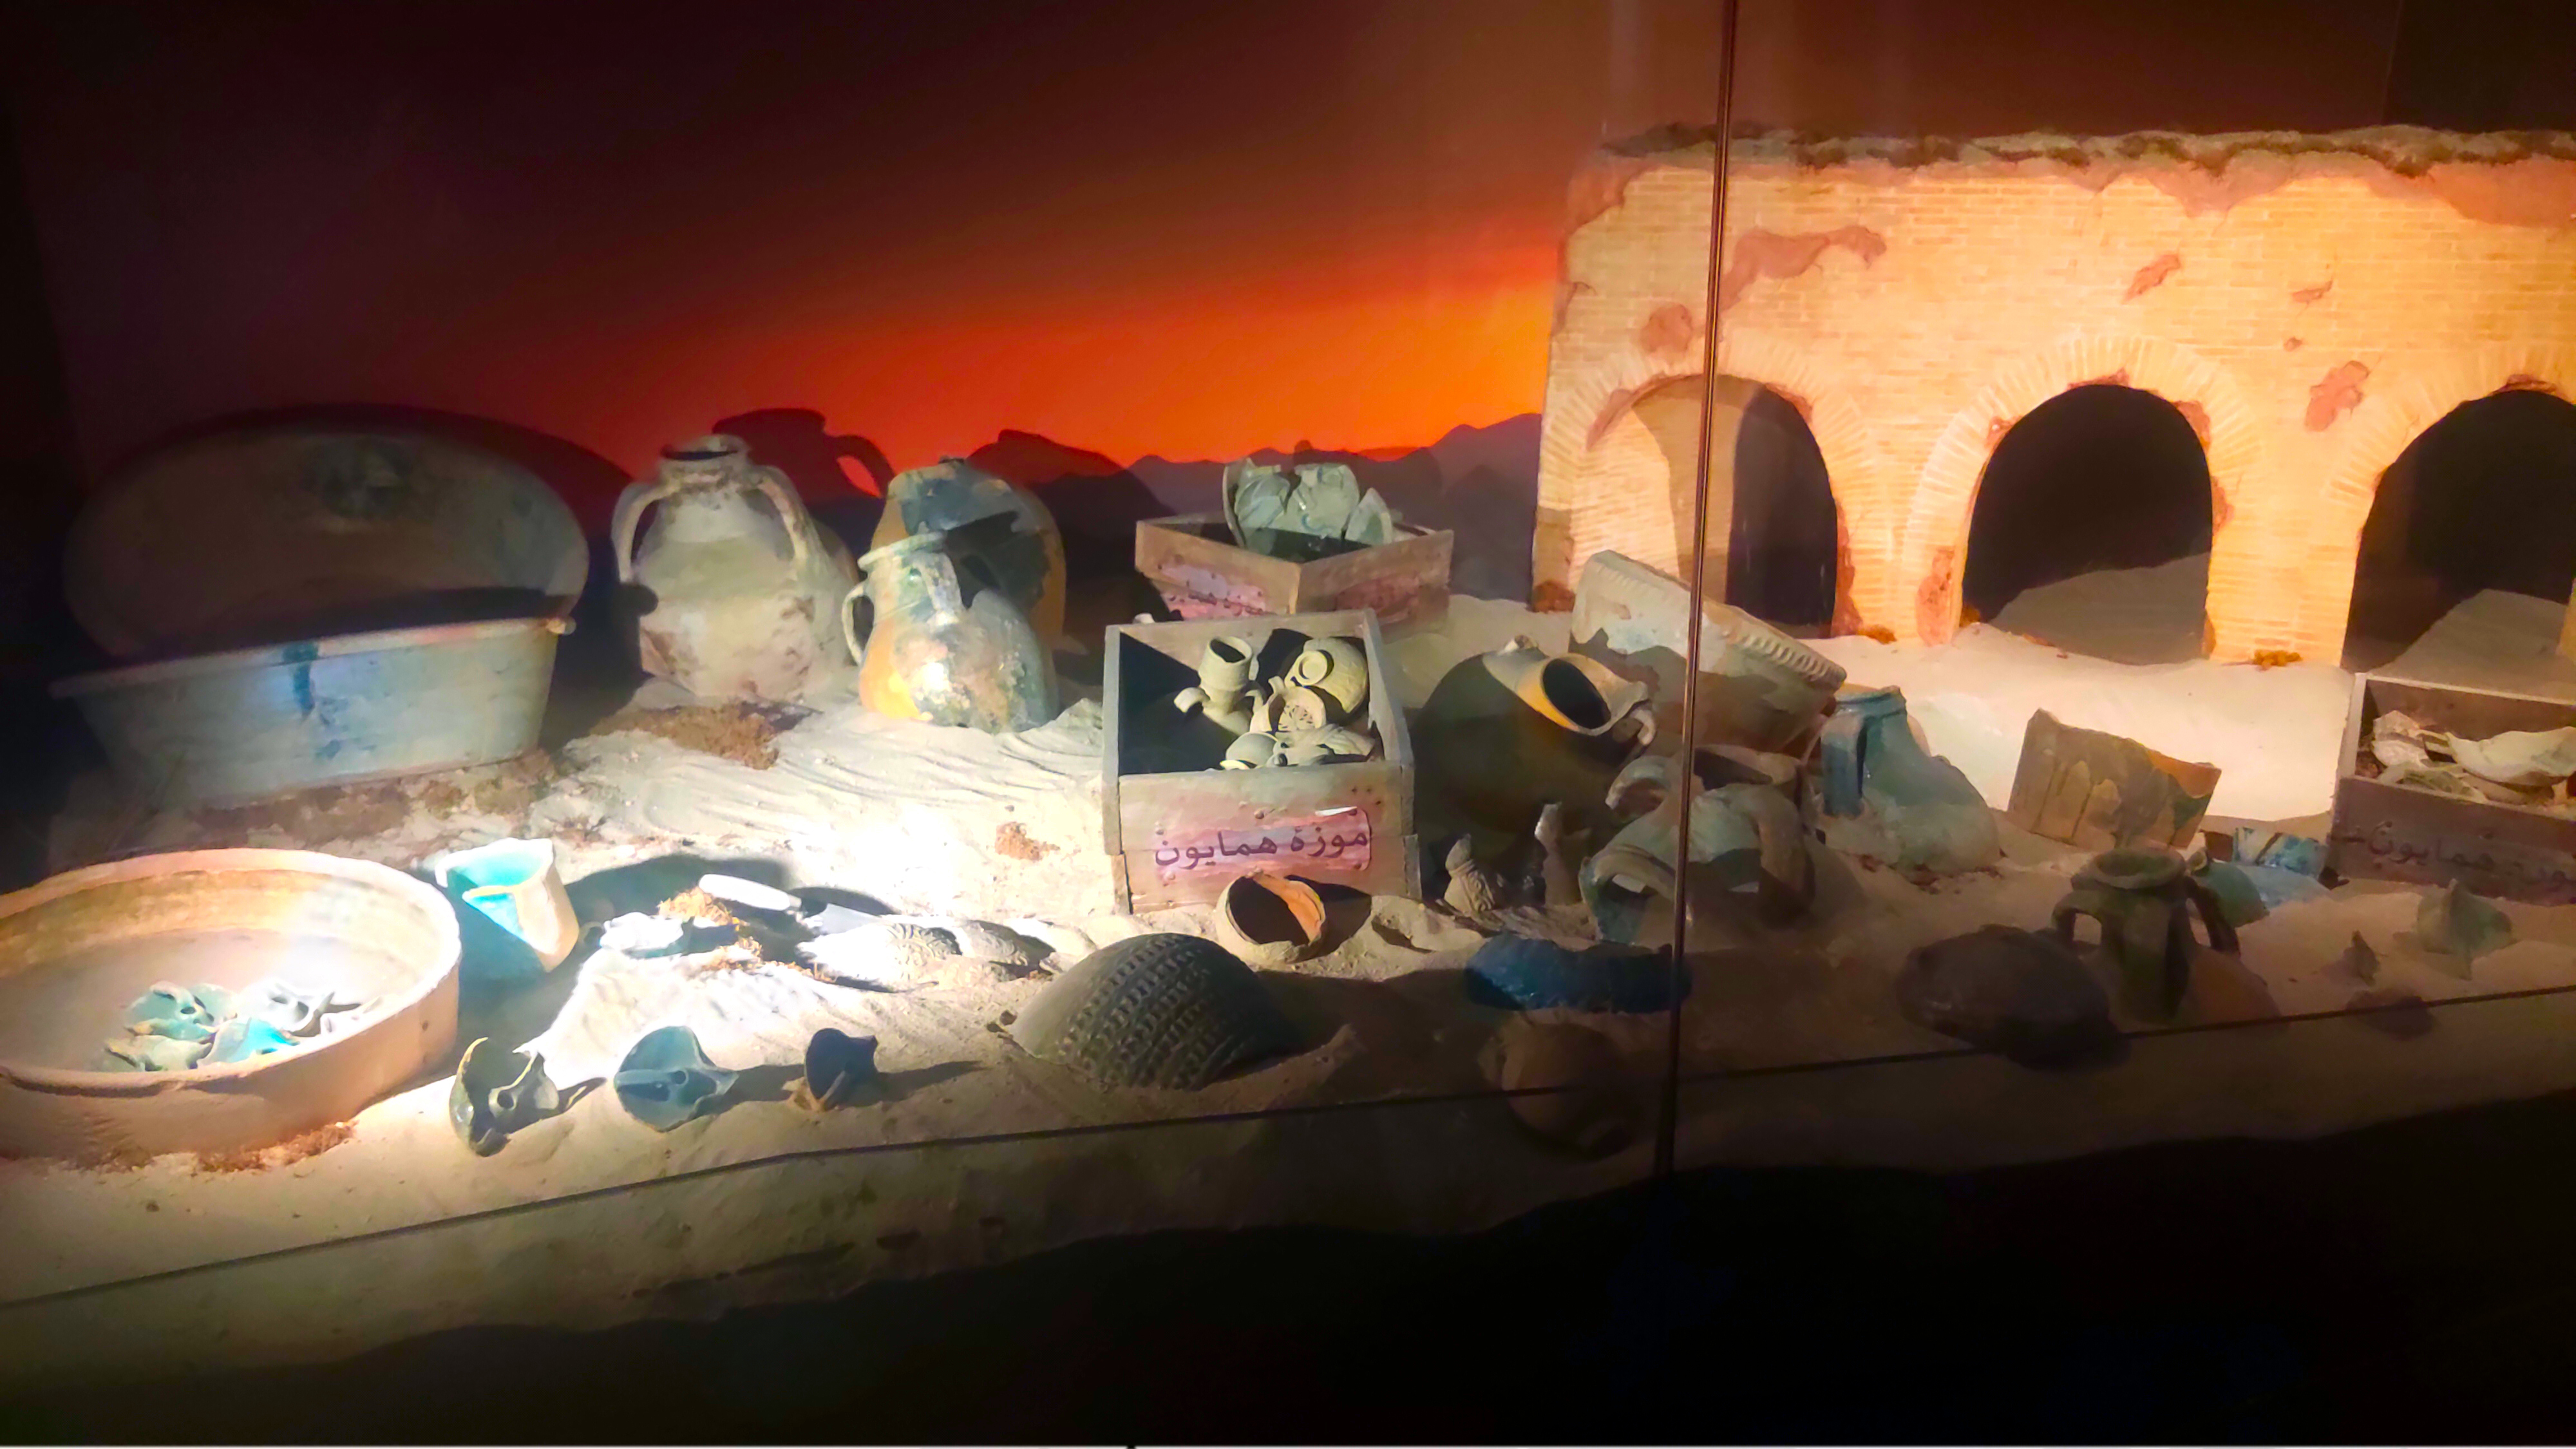
\includegraphics[width=0.4\textwidth]{assets/raqqa.jpg}
    \caption{Rakka Seramikleri}
    \label{fig:raqqa}
\end{wrapfigure}
\indent Lahitler ile kitabeler arasındaki bölümde, Samarra Camii'nin kalıntılarını ve planını gösteren sergi karşımıza çıkıyor. Dönemin Abbasi halifesi el-Mu'tasım'ın ordusu, ağırlıklı olarak Türk askerlerini içerirdi. Bu askerleri başkent Bağdat'ta barındırılması, bir süre sonra hem şehrin güvenliği hem de halkın huzuru üzerinde sorun teşkil etmeye başladı. Bundan dolayı halife el-Mu'tasım, Türk birlikleri yerleştirmek ve askeri üs oluşturmak için, Bağdat'ın 125 kilometre kuzeyine 836 yılında Samarra şehrini kurdu. 848 yılında Abbasi halifesi Mütevekkil tarafından yapımına başlanan Samarra Camii, 852 yılında tamamlanmıştır. 1250 civarında, Moğol akınları sırasında yerle bir edilen camiinin günümüze sadece minaresi ulaşmıştır. İslâm mimarisinde nadir rastlanan bir tarza sahip olan ve Babil zigguratlarını andıran minare, spiral şekilde yükselmektedir. Şehrin bir askeri üs olduğu düşünüldüğünde, minarenin bir istihkâm olarak kullanılması düşünülmüş olabilir.\newline
\indent Kitabelerin bulunduğu odadaki sergide ise Rakka seramikleri bulunmaktadır. Eyyübiler döneminde bölge ekonomisinin temel direğini seramikçilik oluşturmaktaydı. 19. yüzyıl sonlarında yapılan kazılar ile ortaya çıkan Rakka seramik eserleri burada sergilenmektedir. Şekil \ref{fig:raqqa}'de görülen sandıklar üzerinde \textit{Müze-i Hümayûn} yazmaktadır. Eserlerin Türk İslâm Müzesi'nden önceki durağı İstanbul Arkeoloji Müzesi olmalıdır.\newline 
\subsubsection{El Yazması Eserler}
\indent\indent Müzede, 2500 civarında yazma eser bulunmaktadır. El yazmaları, ağırlıklı olarak Kur'an-ı Kerim, cüz ve mecmua tarzı eserleri ihtiva etmektedir.\newline
\indent Müzede Emevi, Memlûk, İlhanlı, Timur, Safevi ve Kaçar dönemlerine ait el yazması Kur'an-ı Kerim ve cüz eserler dönemlerine göre ayrı odalarda tasnif edilmiş halde sergilenmektedir. Bu eserlerden Emevi dönemi el yazması Kur'an-ı Kerim büyüklüğü ile ilgi çekicidir. İlhanlı dönemine ait Kur'an-ı Kerim'de ise tefsir çalışması mevcuttur. Tefsir, satırların altına kırmızı kalem ile işlenmiştir. Memlûk ve Safevi el yazmalarında tezhip(Arapça \textit{zeheb(altın)} kelimesinden altınlamak anlamında) sanatının nadide işçiliği gözlemlenebilir. Şam Emevi Camii'nden 1917 yılında getirilerek, Şam Evrakı koleksiyonu şeklinde sergilenen eserler arasında parşömen üzerine Kur'an sayfaları 846 gibi erken bir tarihe uzanmakta ve İslâm sanatının ilk örneklerini ouşturmaktır. Şam Evrakı Koleksiyonunda Kur'ân yapraklarının yanı sıra, 8. yüzyıl sonundan 19. yüzyıla kadar uzanan bir periyodda yazılmış ciltler ve belgelere de bulunmaktadır.\newline
\indent Kur'an-ı Kerim ve cüz eserlerin yanı sıra az sayıda mecmua eserler de el yazması eserler arasında bulunmaktadır. Bu eserler arasinda Timur döneminden Hamse-i Attar(beş mesneviden oluşan külliyat) ve Memlûk döneminden Kitab-ı Buzuğ El Hilal adında bir mecmua dikkat çekmektedir.
\begin{figure}[H]
    \centering
    \subfigure[Hamse-i Attar]{
        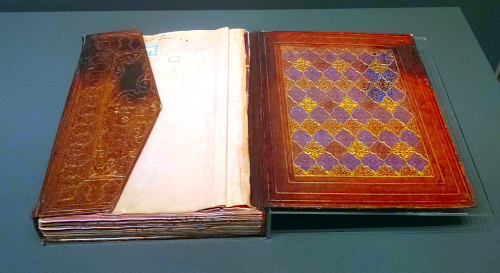
\includegraphics[height=0.2\textheight, width=0.45\linewidth]{assets/hamsei_attar.jpg}
    }
    \hfill
    \subfigure[Kitab-ı Buzuğ El Hilal]{
        \includegraphics[height=0.2\textheight, width=0.45\linewidth]{assets/kitabi_buzug_el_hilal.jpg}
    }
    \caption{El Yazması Mecmua Eserler}
\end{figure}
\begin{figure}[H]
    \centering
    \subfigure[İlhanlı Dönemi Kur'an Kerim ve Tefsir Çalışması]{
        \includegraphics[width=0.9\linewidth]{assets/ilhanli_kuran_tefsir.jpg}
        \label{fig:ilhanli_tefsir}
    }
    \vspace{10pt}
    \subfigure[Emevi Dönemi Kur'an-ı Kerim]{
        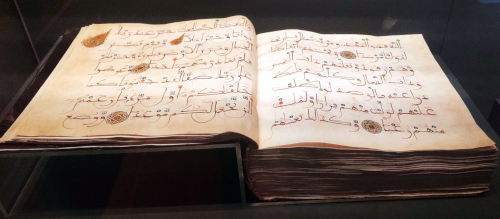
\includegraphics[height=0.2\textheight, width=0.45\linewidth]{assets/emevi_kuran.jpg}
        \label{fig:emevi}
    }
    \hfill
    \subfigure[Memlûk Dönemi Kur'an-ı Kerim]{
        \includegraphics[height=0.2\textheight, width=0.45\linewidth]{assets/memluk_kuran.jpg}
        \label{fig:memluk_kuran}
    }
    \vspace{10pt}
    \subfigure[Safevi Dönemi Kur'an-ı Kerim]{
        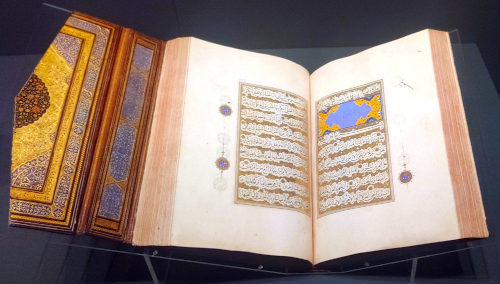
\includegraphics[height=0.2\textheight, width=0.45\linewidth]{assets/safevi_kuran.jpg}
        \label{fig:safevi_kuran}
    }
    \subfigure[Kaçar Dönemi Kur'an-ı Kerim]{
        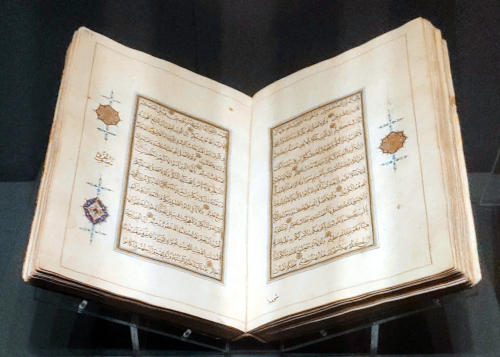
\includegraphics[height=0.2\textheight, width=0.45\linewidth]{assets/kacar_kuran_mesnevi.jpg}
        \label{fig:kacar_kuran_mesnevi}
    }
    \caption{El Yazması Kur'an-ı Kerim ve Cüz Eserler}
    \label{fig:quran}
\end{figure}
\subsubsection{Kutsal Emanetler}
\begin{wrapfigure}{r}{0.25\textwidth}
    \centering
    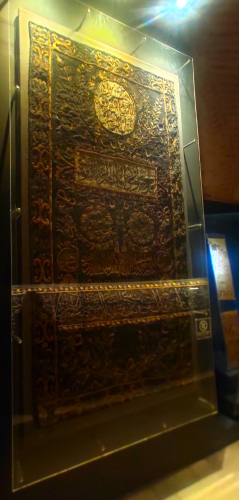
\includegraphics[width=0.20\textwidth]{assets/kabe.jpg}
    \caption{Kabe Örtüsü}
    \label{fig:kabe}
\end{wrapfigure}
\indent\indent Müzede, kutsal emanetler için ayrı bir bölüm oluşturulmuş. Burada dikkat çeken eserlerin başında Kâbe örtüsü bulunmaktadır. Hz. Ömer zamanında başlayan bir gelenek olarak Kâbe örtüsü masrafları devlet hazinesinden karşılanıyordu. Memlûk sultanları döneminde bu örtünün dokunması Mısır'da yapılmaya başlandı. 1517 yılında Yavuz Sultan Selim Mısır'ı fethendice, eski usûle bağlı kalarak örtünün Mısır'da dokunmasını buyurdu. Kanuni Sultan Süleyman zamanında dış örtünün Mısır'da, iç örtünün ise İstanbul'da dokunması kararlaştırıldı. III. Ahmed döneminden itibaren hem iç, hem de dış örtü İstanbul'da dokunmaya başlandı. Sultan Abdülaziz'in 1861'de tahta çıkması münasebetiyle gönderilen örtü, 1943 yılına kadar kullanıldı. I. Dünya Savaşı sırasında bölgenin Osmanlı Devleti'ne karşı ayaklanması ile örtülerin dokuması Mısır'da yapılmaya başlanmıştır. 1962 yılından itibaren örtülerin dokuması Mekke'de kurulmuş fabrikada yapılmaktadır.\cite{dia_4}\newline
\indent Bu kısımdaki bir diğer ilgi çekici eser ise hac vekaletnameleridir. Günümüzde de uygulanmaya devam eden vekalet ile hac uygulaması, geçmişte daha sık başvurulan yöntemdi. Hac yapmakla mükellef kişi bir sağlık sorunu, yaşlılık gibi sebeplerden dolayı başka bir kişiyi vekil olarak gönderebilmektedir. İşte bu vekilliği belgeyen vekaletnamelerin nüshaları burada incelenebilmektedir.\newline
\indent İç kısımda ise el yazmaları bulunmaktadır. Burada el yazması Kur'ân-ı Kerimlerden bir tanesinin Hz. Osman döneminde, bir diğerinin ise Hz. Ali döneminde yazıldığı rivayet edilmektedir. Yine Aşere-i Mübeşşere'nin(Hz. Muhammed tarafından cennetle müjdelenen on kişi) isimlerinin yazılı olduğu örtü de bu alanda sergilenmektedir. Bunların dışında eski bir Kâbe kapısı kilidi ve Kâbe mührü gibi eserler de burada görülebilir.
\begin{figure}[H]
    \centering
    \subfigure[Hz. Osman Dönemi Kur'ân-ı Kerim]{
        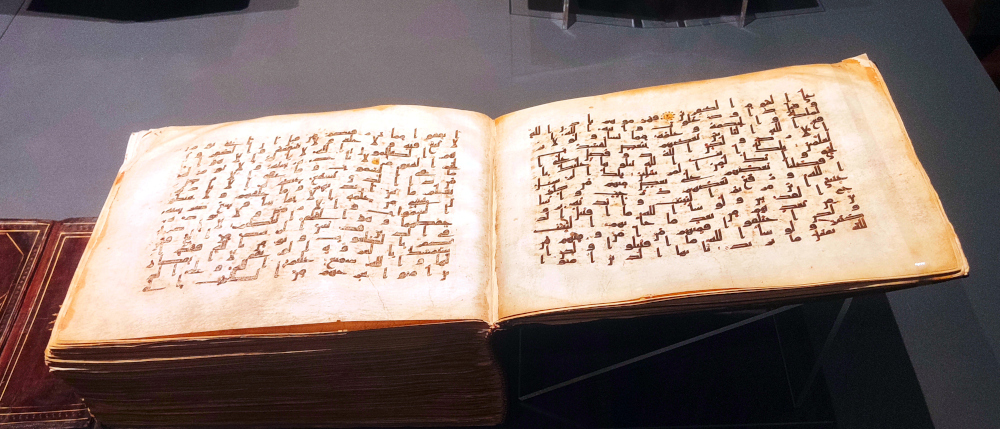
\includegraphics[height=0.2\textheight, width=0.45\linewidth]{assets/osman.jpg}
    }
    \hfill
    \subfigure[Hz. Ali Dönemi Kur'ân-ı Kerim]{
        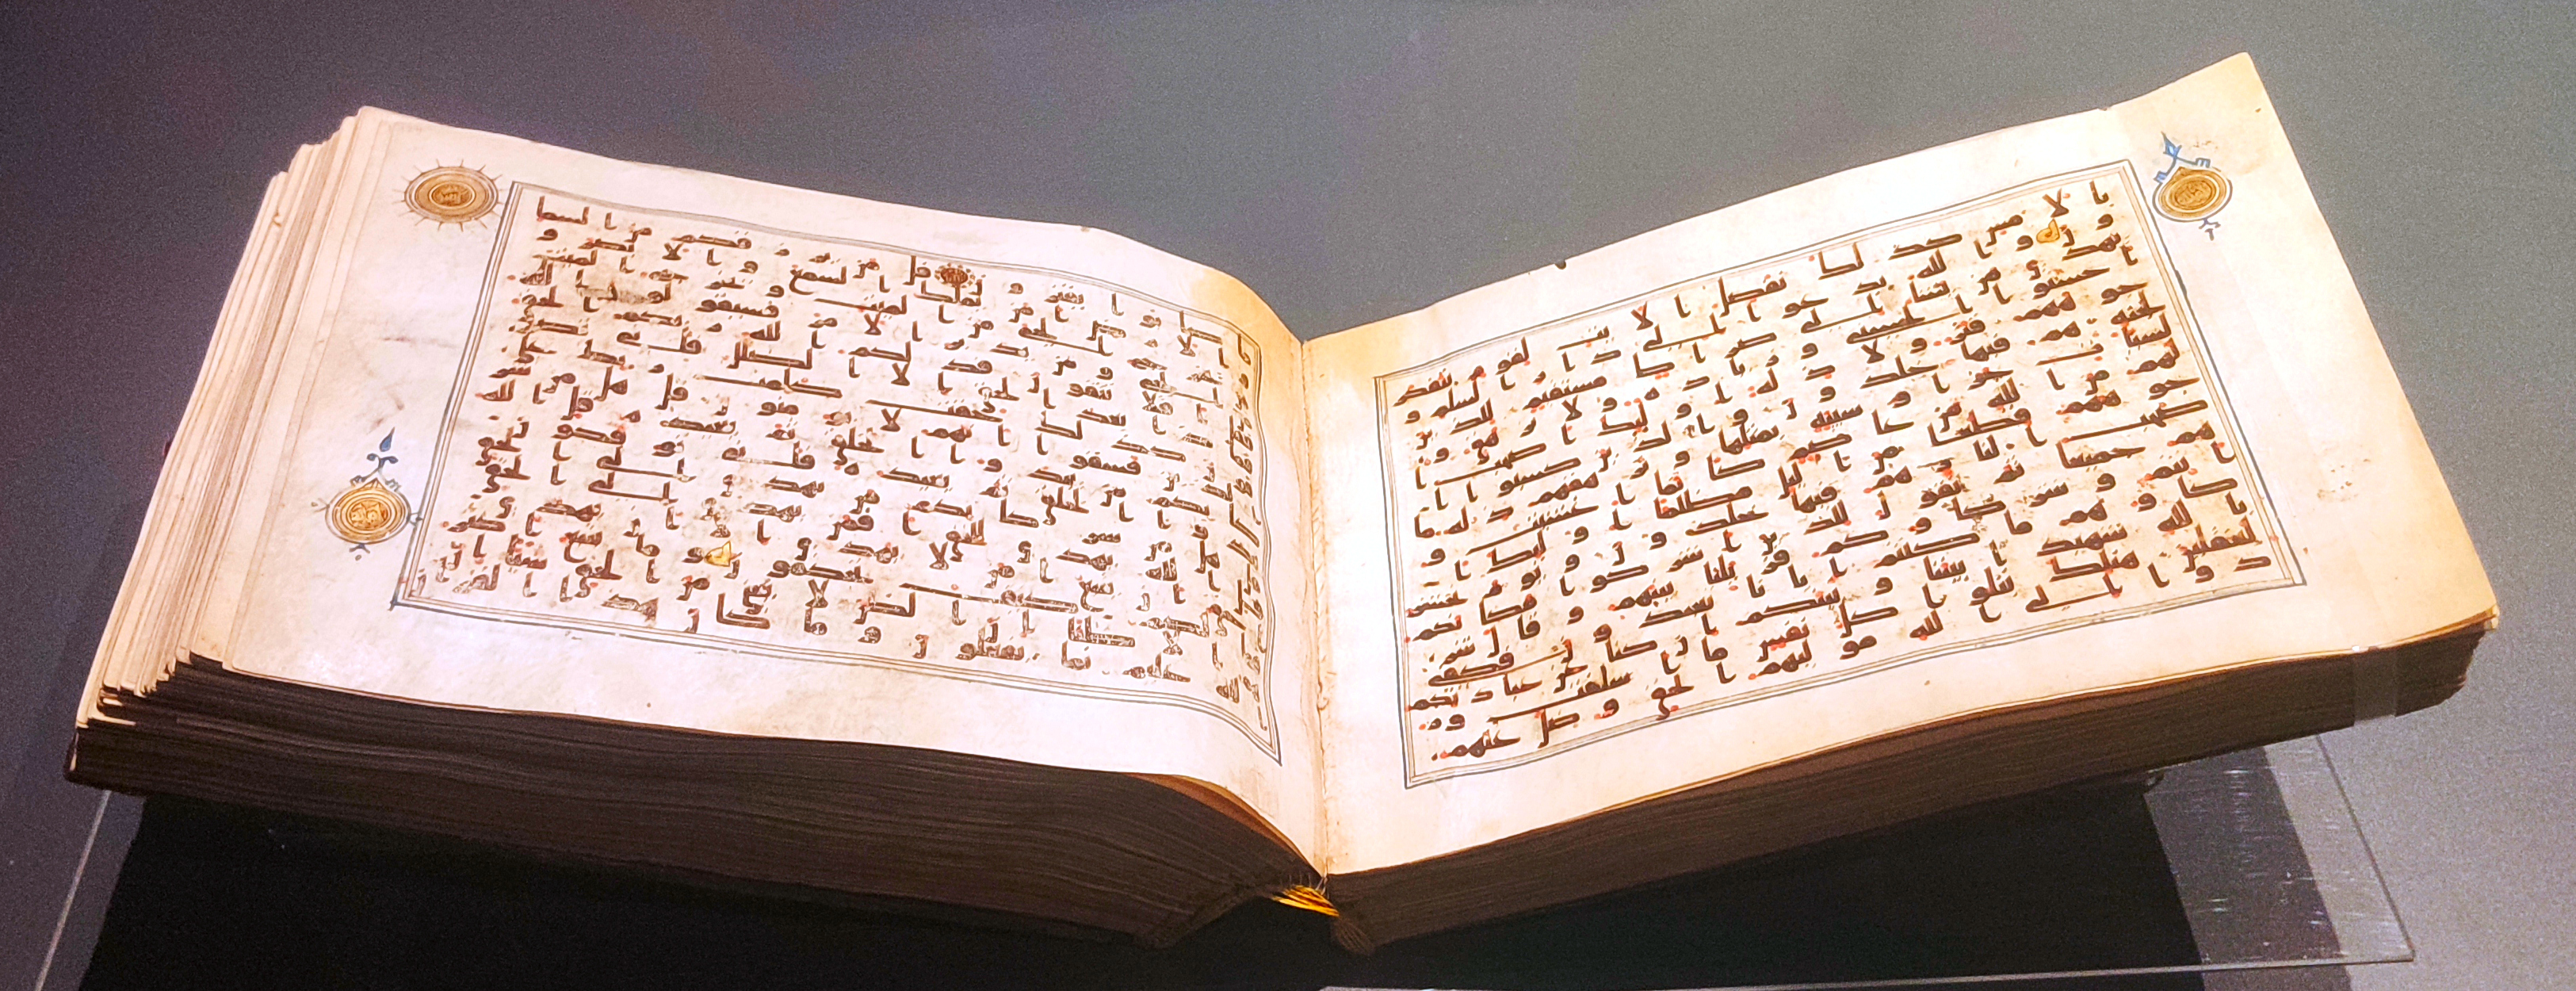
\includegraphics[height=0.2\textheight, width=0.45\linewidth]{assets/ali.jpg}
    }
    \caption{Halife Dönemi El Yazması Kur'ân-ı Kerimler}
\end{figure}
\subsubsection{Diğer Eserler}
\begin{wrapfigure}{r}{0.3\textwidth}
    \centering
    \includegraphics[width=0.3\textwidth]{assets/cizre.jpg}
    \caption{Ulucamii Kapısı}
\end{wrapfigure}
\indent\indent Müzede dikkat çeken bir başka eser ise Cizre Ulucamii kapısıdır. Cizre Ulucamii, Abbasiler döneminde kiliseden camiiye çevrilmiş ve tamir edilmiştir. Artuklular döneminde(1160) yeniden inşa ettirilmiştir. Kapıları 1946 yılında onarılmış ve yapı 2007 yılında Vakıflar Genel Müdürlüğü tarafından restore edilmiştir. Cizre Ulucamii'nin en dikkat çekici unsuru bronzdan yapılmış kapısı ve tokmaklarıdır. Tokmaklar, iki ejderin arasında bir aslan başı şeklinde tasarlanmıştır. Tokmaklardan biri, 1969 yılında yurt dışına kaçırılmıştır.\cite{dia_5}\newline
\indent Müzede, çeşitli dönemlere ait şamdanlar, buhurdanlıklar, yağdanlıklar, seramik eşyalar, keşküller(yarımküre biçiminde bir tür tas), erken dönem astronomik aletler de bulunmakta. Büyük Selçuklular dönemine ait tabure, matara ve reçellikler, yıllar geçse de insanların ihtiyaçlarının aşağı yukarı aynı kaldığını gösteriyor bizlere. Yine aynı galeride bulunan Selçuklu seramik yıldızının örnekleri, Konya Karatay Medresesi Müzesi'nde de bolca bulunmaktadır. Bir diğer ilginç eser ise Kaçar döneminden kalma lakeden yapılmış oyun kartları ve kalemliklerdir. Oyun kartları, Antik Mısır'da oynanan \textit{Senet} oyununun bir benzeri gibi durmaktadır. Fakat aradaki yaklaşık 5000 yıllık zaman farkını düşününce, bu ihtimal çok ufaktır.
\newpage
\clearpage
\begin{figure}[!ht]
    \centering
    \subfigure[Selçuklu Dönemi Seramikleri]{
        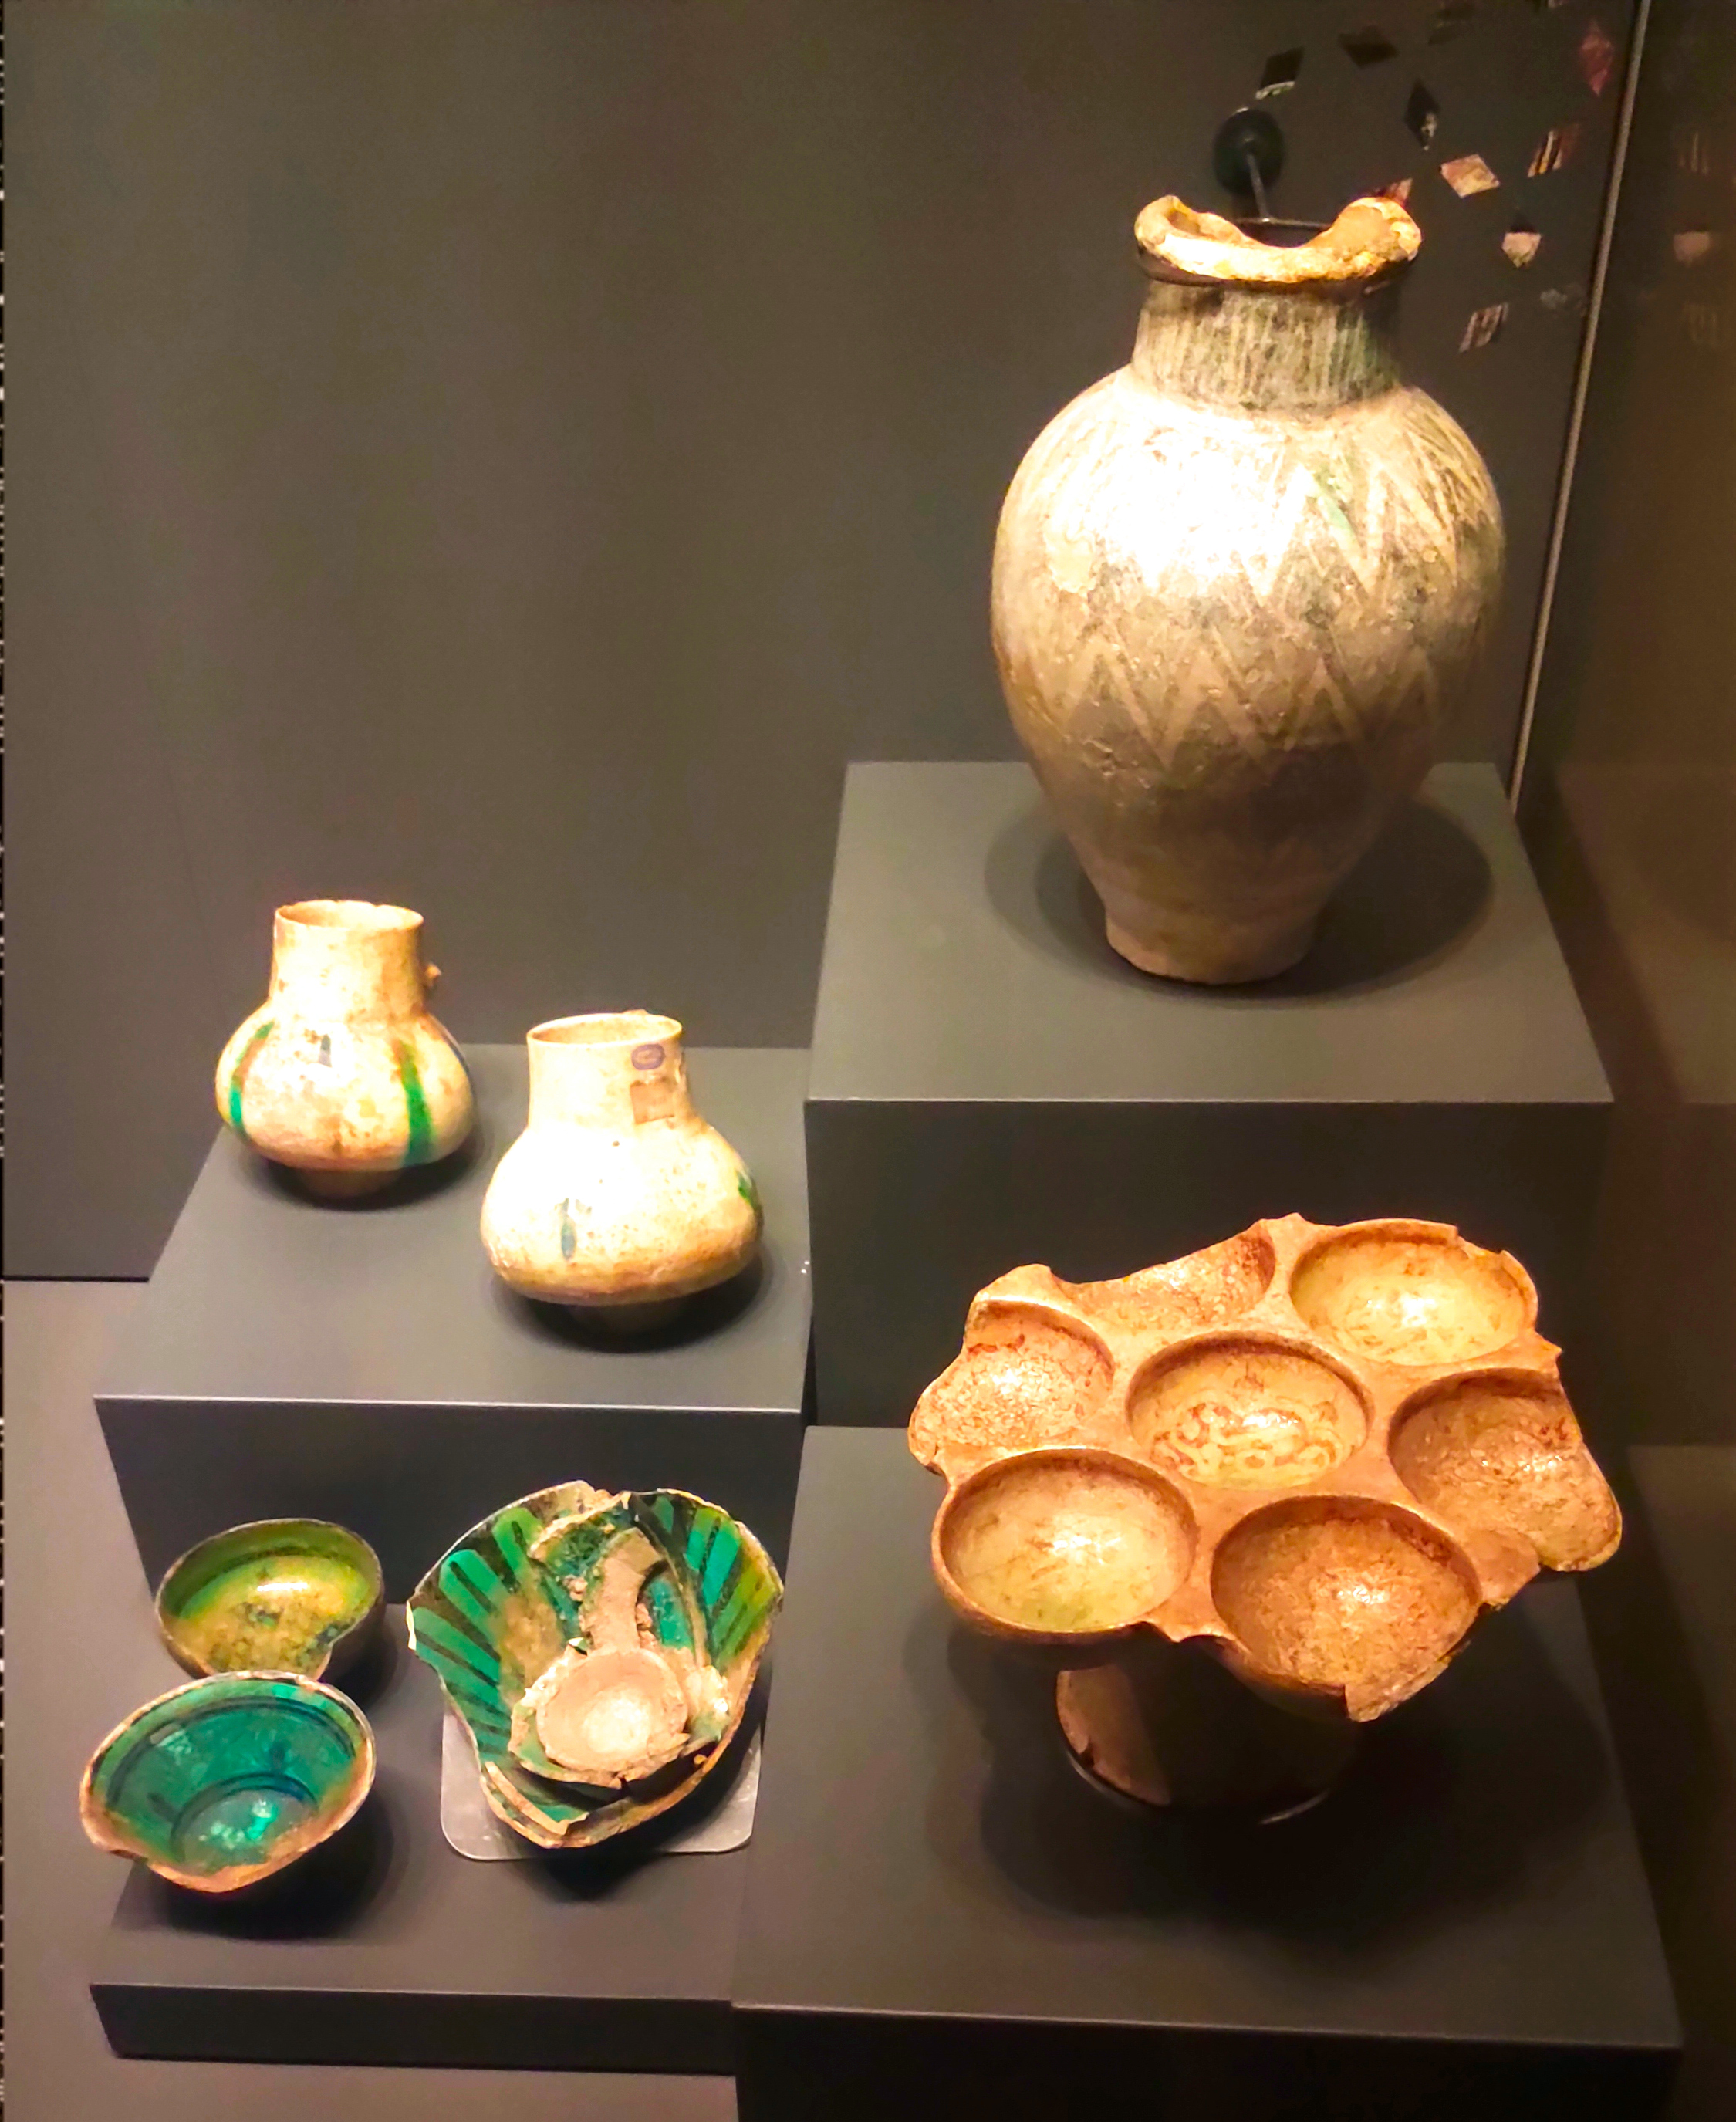
\includegraphics[height=0.25\textheight, width=0.3\linewidth]{assets/seljuks_1.jpg}
        \label{fig:seljuks_1}
    }
    \hfill
    \subfigure[Selçuklu Dönemi Seramikleri]{
        \includegraphics[height=0.25\textheight, width=0.3\linewidth]{assets/seljuks_2.jpg}
        \label{fig:seljuks_2}
    }
    \hfill
    \subfigure[Selçuklu Dönemi Seramikleri]{
        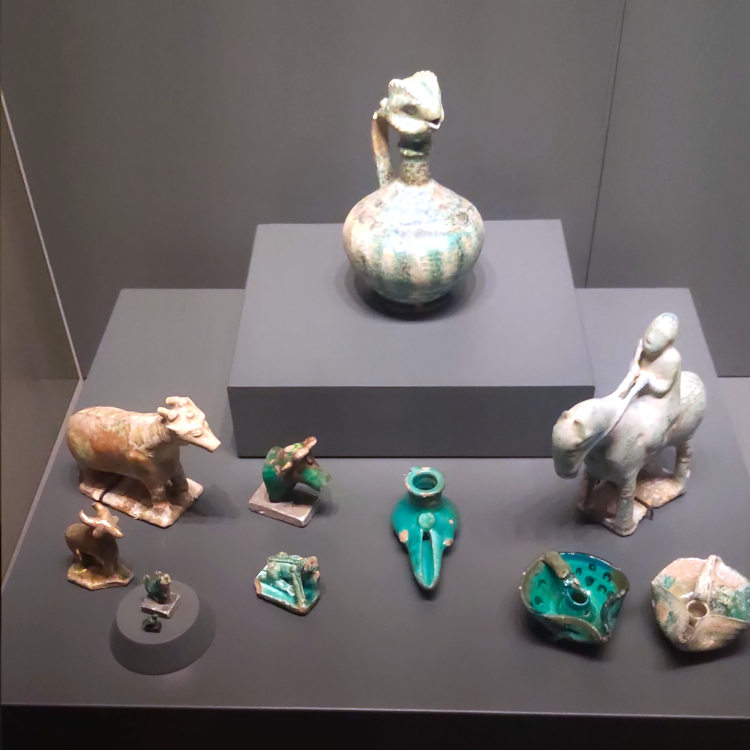
\includegraphics[height=0.25\textheight, width=0.3\linewidth]{assets/seljuks_4.jpg}
        \label{fig:seljuks_4}
    }
    \vspace{10pt}
    \subfigure[Selçuklu Seramik Yıldızı]{
        \includegraphics[height=0.25\textheight, width=0.3\linewidth]{assets/seljuks_3.jpg}
        \label{fig:seljuks_3}
    }
    \hfill
    \subfigure[Kaçar Dönemi Kalmlikler]{
        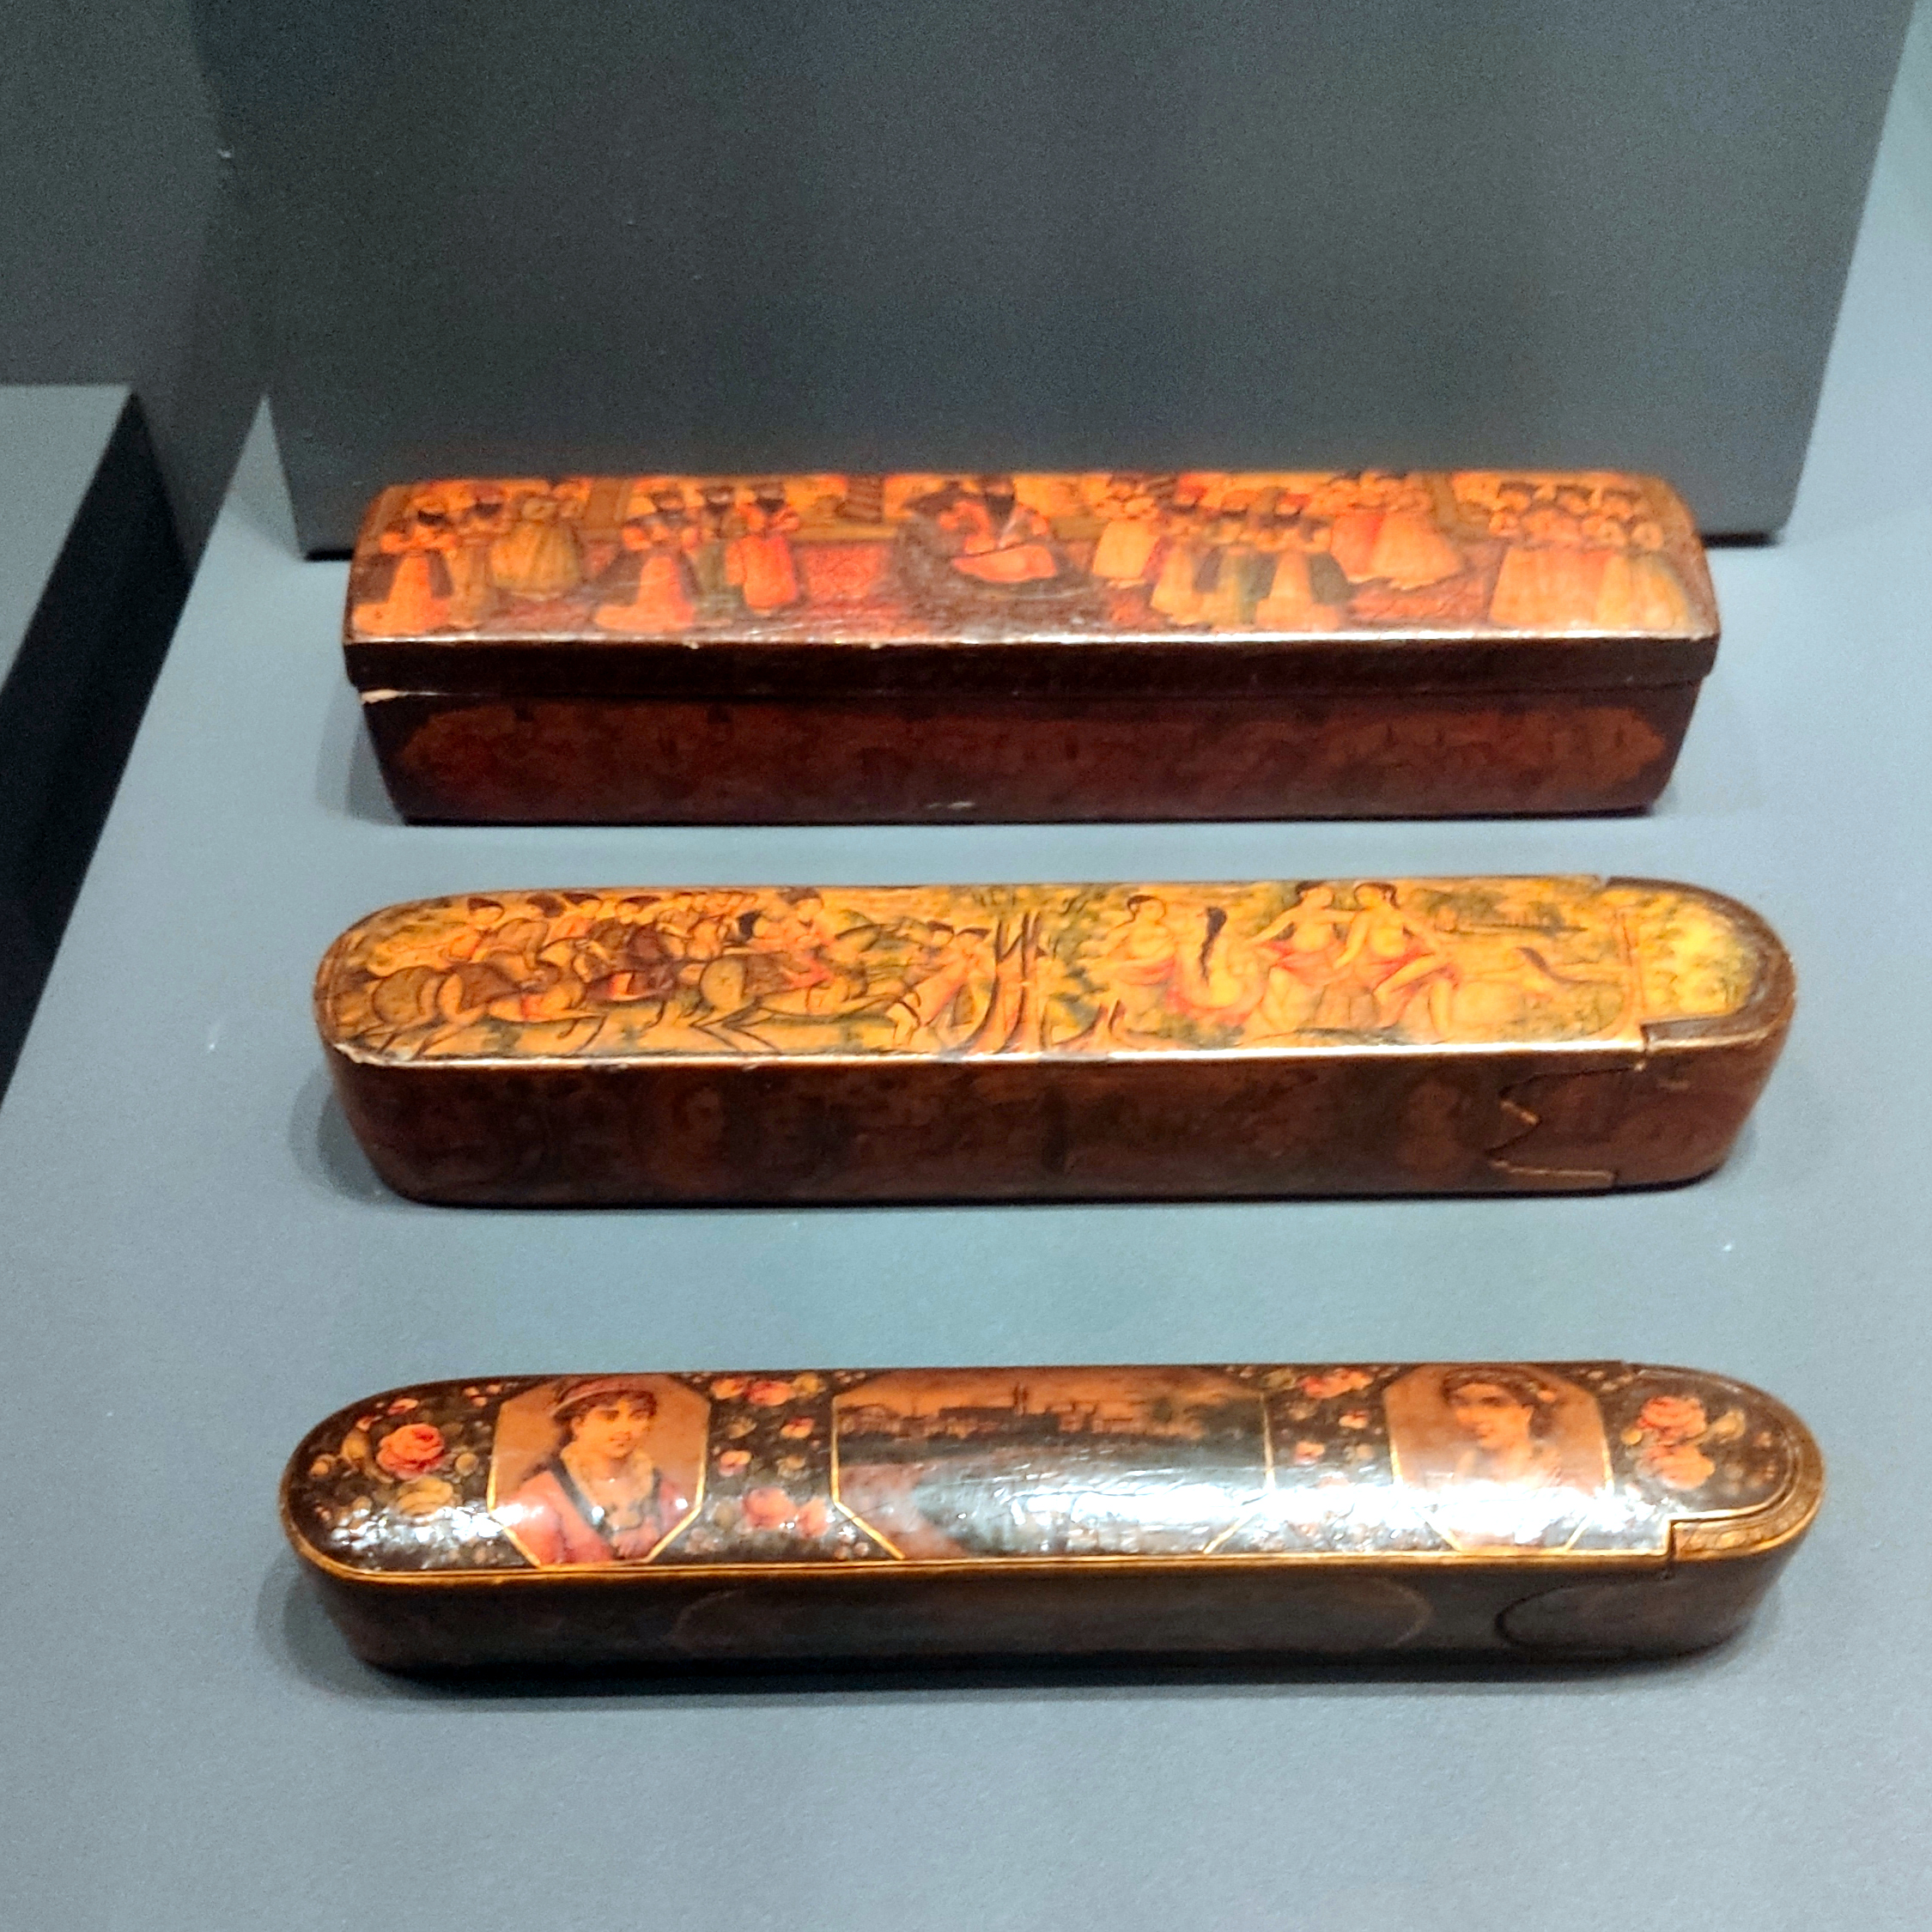
\includegraphics[height=0.25\textheight, width=0.3\linewidth]{assets/qajars_1.jpg}
        \label{fig:qajar_1}
    }
    \hfill
    \subfigure[Kaçar Dönemi Lake Oyun Kartları]{
        \includegraphics[height=0.25\textheight, width=0.3\linewidth]{assets/qajars_2.jpg}
        \label{fig:qajar_2}
    }
    \caption{Diğer Eserler}
    \label{fig:other_pieces}
\end{figure}
\section{Üçüncü Hafta  - Türk İslam Eserleri Müzesi}
\indent\indent Müze uzmanlarından Tarık Akar tarafından müzenin alt katındaki sergi alanları gezilip, müzede sergilenen eserler hakkında bilgi verildi. 
\subsection{Anadolu Selçuklular Galerisi}
\indent\indent Müzenin bu kısmında Anadolu Selçuklu dönemine ait halı ve kilimleri geniş yer kaplıyor. 13.yüzyıldan kalma olan eserler, Anadolu'nun en eski halı ve kilim örneklerini oluşturmaktadır. Salonun ortasındaki vitrinde ise Anadolu Selçuklu döneminden kalma maşrapalar, vazolar, mataralar ve sürahiler bulunmaktadır. Bunlarla birlikte, yine bu döneme ait savaşçı ve grifon figürlü mermer kabartmalar bulunmaktadır.\newline
\begin{figure}[H]
    \centering
    \subfigure[Grifon Kabartması]{
        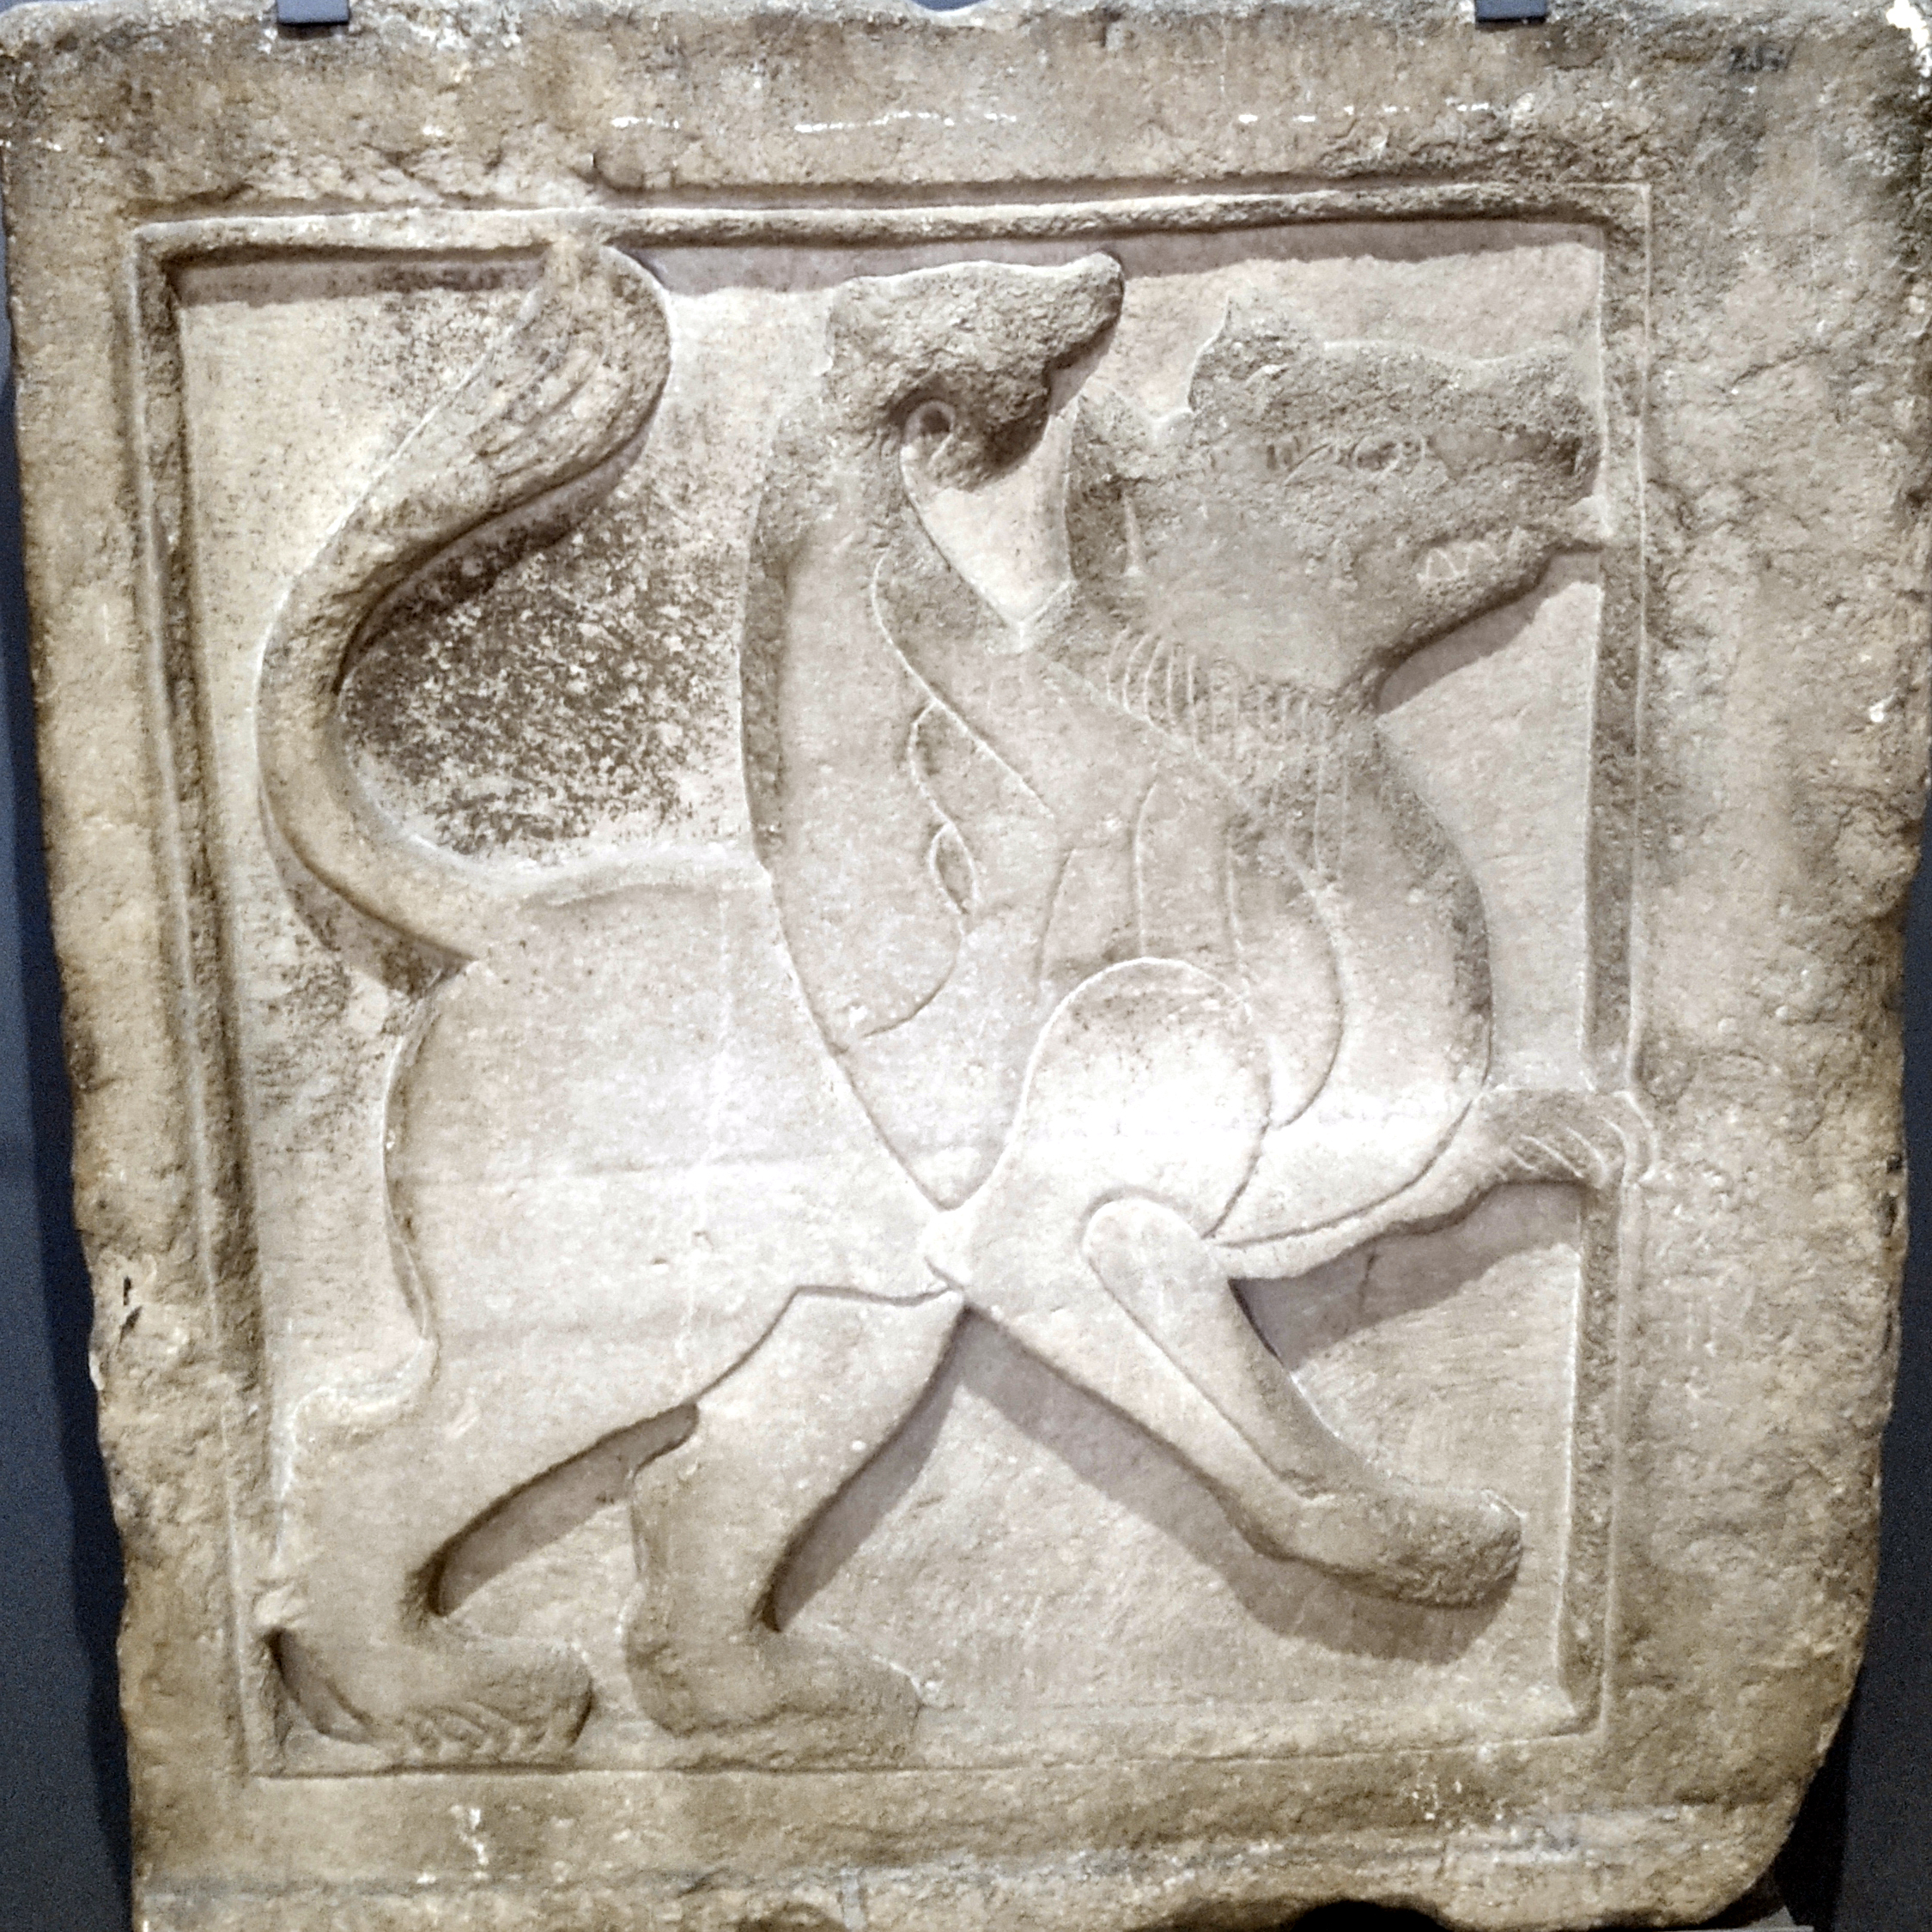
\includegraphics[height=0.3\textheight,width=0.3\textheight,keepaspectratio=false]{assets/grifon_as.jpg}
    }
    \subfigure[Savaşçı Kabartması]{
        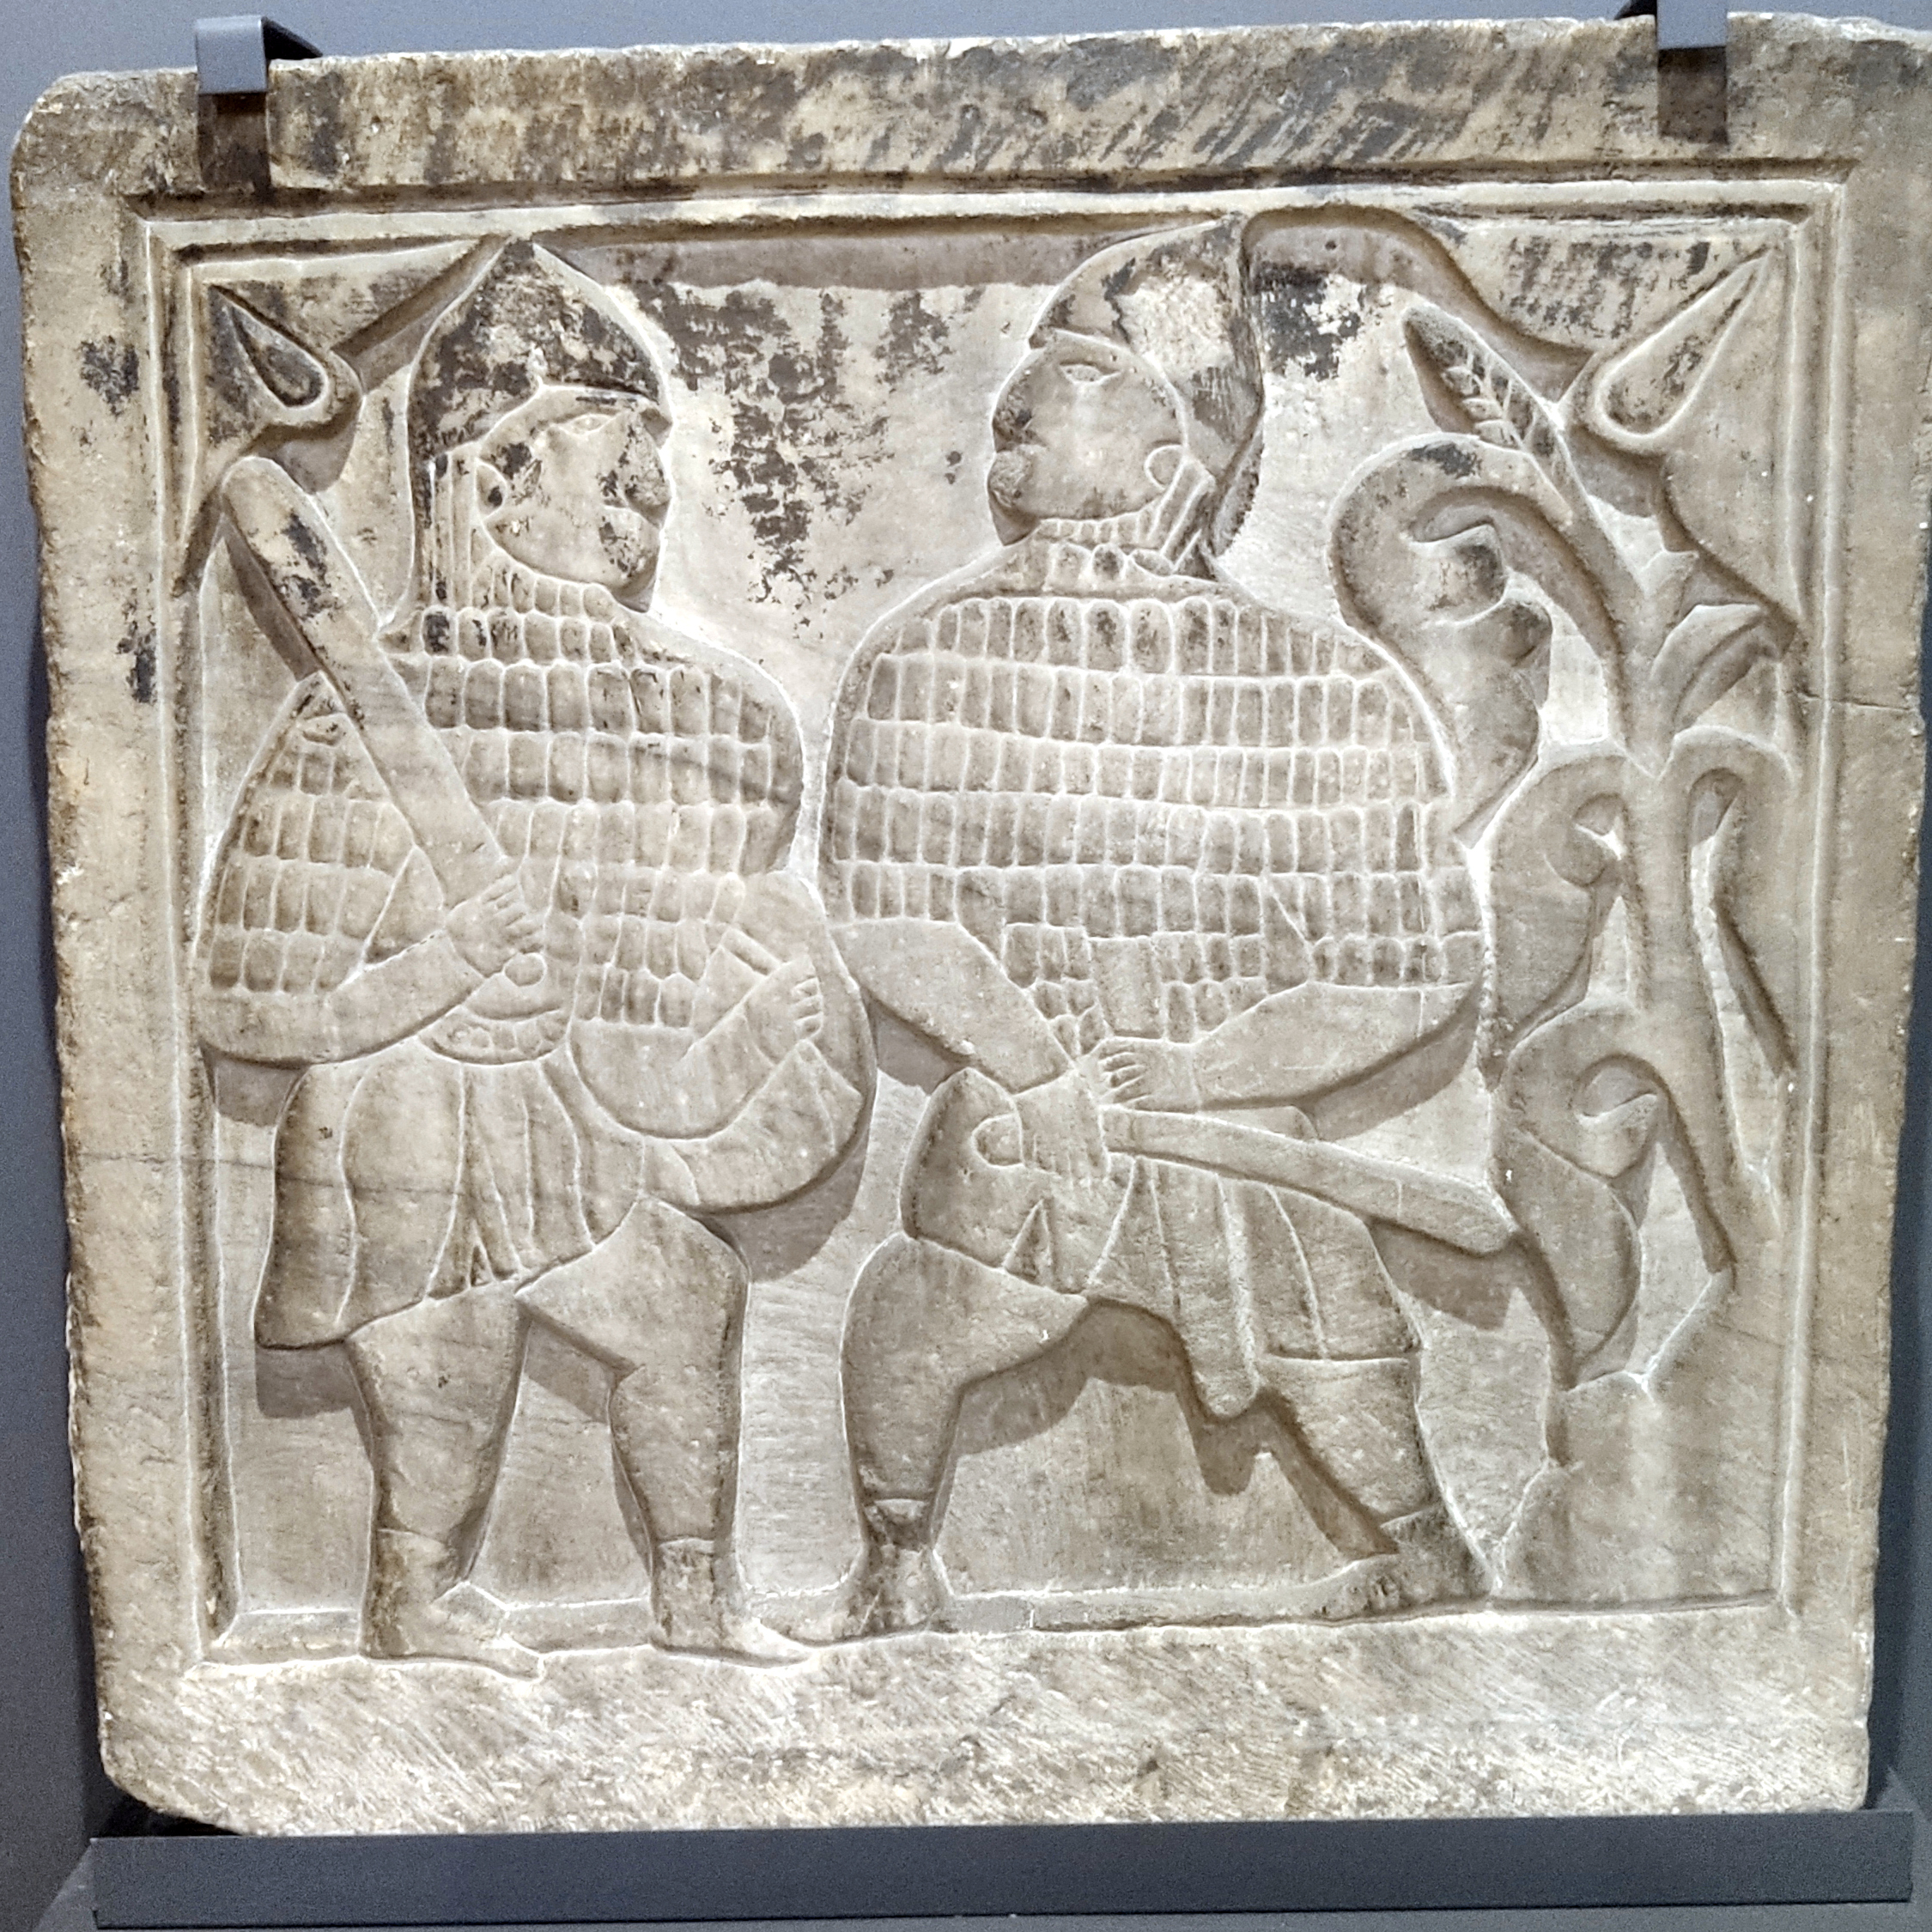
\includegraphics[height=0.3\textheight,width=0.3\textheight,keepaspectratio=false]{assets/savasci_as.jpg}
    }
    \caption{Anadolu Selçuklu Dönemi Mermer Kabartmalar}
\end{figure}
\indent Buradaki ahşap eserler arasında Karamanoğlu İbrahim Bey İmareti'nin kapısı da bulunmakta. Karamanoğlu Beyi II.İbrahim Bey tarafından yaptırılan imaretin vakfiyesi Haziran 1432, kitabesi ise Eylül 1432 tarihlidir. Bu kapı ceviz ağacından yapılmıştır. Sağ kanat üzerinde \textit{"Karamanlı neccâr İlyas oğlu Hacı Ömer'in işidir"} yazılıdır. Sol kanattaki benzer yazıdan ise sadece \textit{"neccâr"} kısmı okunmaktadır. Kapıda dikkat çeken unsur ise sol kanattaki ahşap işçiliğinin sağ kanada oranla daha göz alıcı olmasıdır. Yine aynı imarete ait pencere kanatları da hemen kapının sol tarafında bulunmaktadır. Pencere kanadının sol kanadı da ceviz ağacından yapılmıştır. Bu kapı ve pencere kanatlarındaki ahşap işçilikleri Anadolu Selçuklu ve beylikler döneminin en nadide örneklerinden biridir.\cite{dia_6}\newline
\indent Ahşap eserlerden bir diğeri ise, Andaolu Selçuklu döneminin meşhur sufilerinden Seyyid Mahmûd-i Hayrâni'nin Akşehir'deki türbesinden getirilen sandukalardır. Türbede Hayranî, kardeşi ve oğluna ait sandukalar, 20.yüzyıl başlarında yurt dışına kaçırılmak üzere çalınıyor. Eserlerden ikisi yurt dışına çıkmadan yakalansa da, bir tanesi günümüzde Kopenhag'daki David Sampling müzesinde sergilenmektedir.
\begin{figure}[H]
    \centering
    \subfigure[Kapı]{
        \includegraphics[height=0.4\textheight]{assets/ahsap_kapi_karaman_ibrahim.jpg}
    }
    \subfigure[Pencere]{
        \includegraphics[height=0.4\textheight]{assets/karaman_ibrahim_window.jpg}
    }
    \caption{Karamanoğlu İbrahim Bey İmareti'nin Kapı ve Penceresi}
\end{figure} 
\subsection{Osmanlılar Galerisi}
\indent\indent Müzede en büyük kısım Osmanlı dönemi eserlere ayrılmıştır. Bu salonda ağırlıklı olarak Osmanlı dönemi kilimleri ve halıları bulunmaktadır. Bu halı ve kilimler arasında Holbein, Lotto ve Bellini isimleri göze çarpmaktadır. Mezkur ressamlar, eserlerinde Türk halılarını resmettiğinden dolayı, benzer motifli halılar ressamların isimleri ile anılmaktadır. 15. ve 16.yüzyılda halı kullanımı Avrupa'da yaygın olmadığı için, bu halıları zaman zaman masaların üzerine serilmiş şekilde görebiliyoruz resimlerde. Holbein halılarının ana özelliği, sekizgen şeklinde madalyonlardan ihtiva etmesidir. Hans Holbein'in eseleri ve müzedeki halıların karşılaştırması aşağıda görülebilir. (Şekil \ref{fig:holbein})\newline
\begin{figure}[H]
    \centering
    \subfigure[Somerset Ev Konferansı(1604) - Hans Holbein]{
        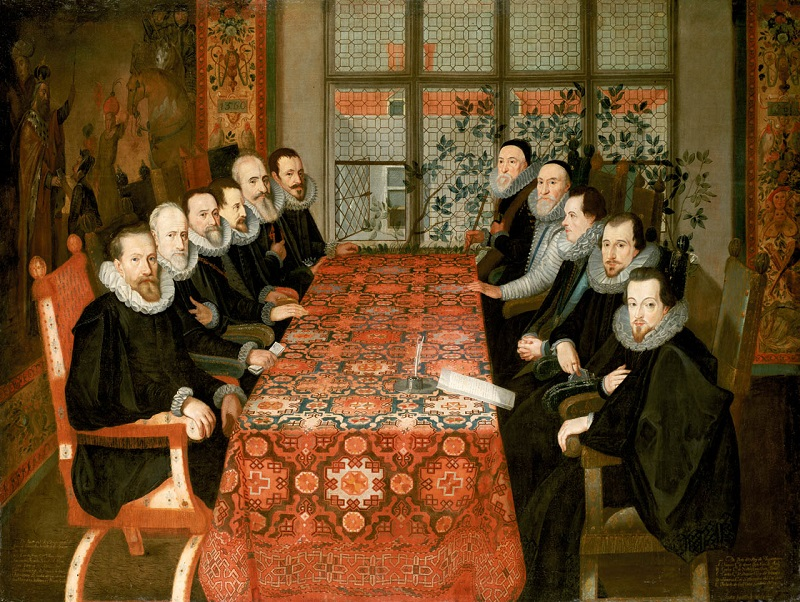
\includegraphics[height=0.3\textheight,width=0.45\linewidth]{assets/somerset_house_conference.jpg}
    }
    \hfill
    \subfigure[Elçiler - Hans Holbein]{
        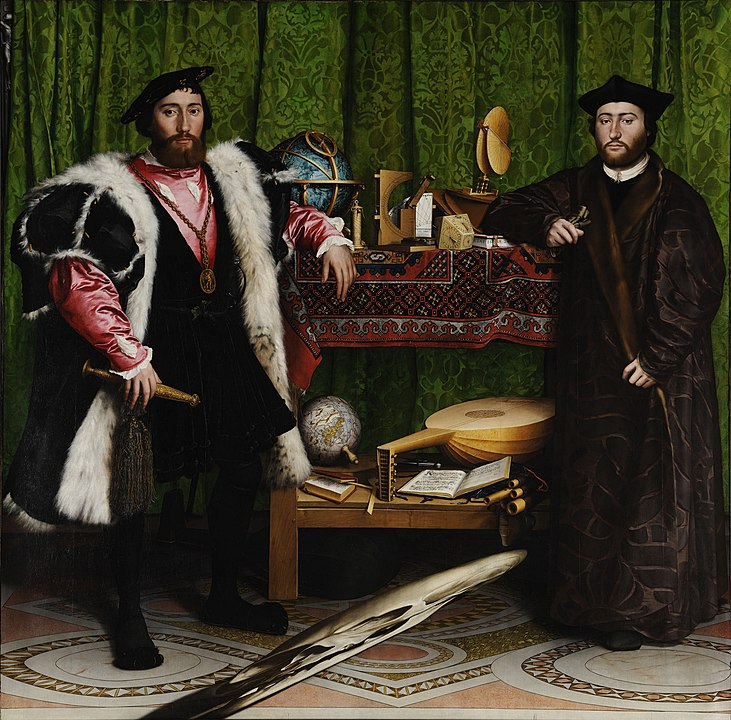
\includegraphics[height=0.3\textheight,width=0.45\linewidth]{assets/envoy.jpg}
    }
    \vspace{10pt}
    \subfigure[Holbein Halısı - 1]{
        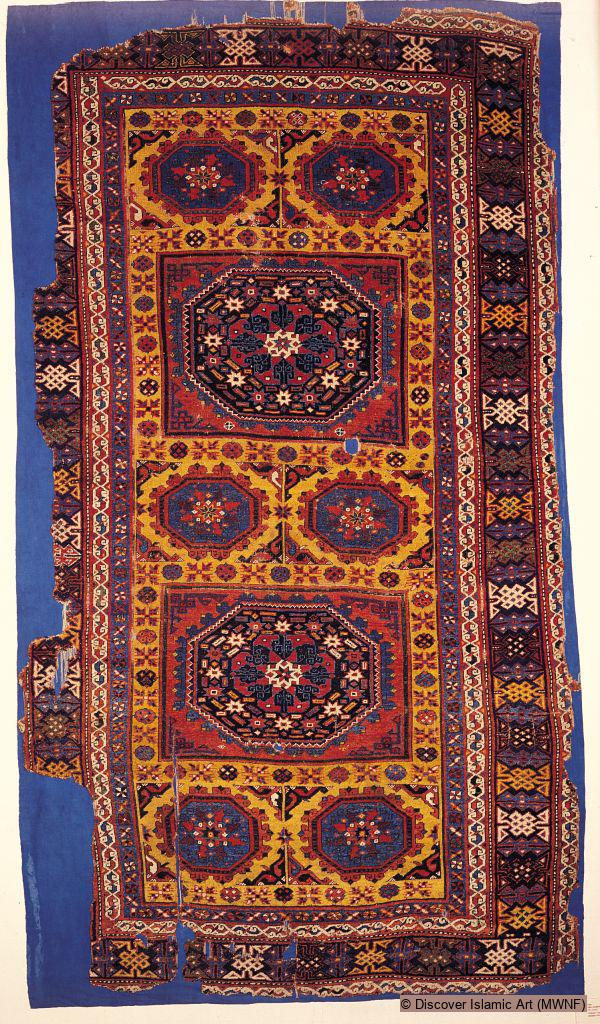
\includegraphics[height=0.3\textheight,width=0.30\linewidth]{assets/holbein_1.jpg}
    }
    \hfill
    \subfigure[Holbein Halısı - 2]{
        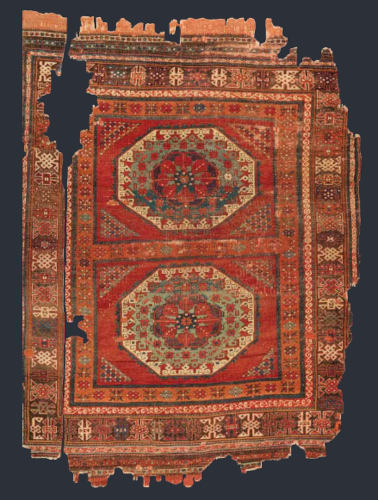
\includegraphics[height=0.3\textheight,width=0.30\linewidth]{assets/holbein_2.png}
    }
    \hfill
    \subfigure[Holbein Halısı - 3]{
        \includegraphics[height=0.3\textheight,width=0.30\linewidth]{assets/holbein_3.jpg}
    }
    \caption{Holbein Resimleri ve Halıları Karşılaştırmalı}
    \label{fig:holbein}
\end{figure}
\indent Yine bu salonda Osmanlı dönemi el yazması eserler, fermanlar ve kuburlar sergilenmektedir. El yazması eserler arasında en ilgi çekici olanı ise \textit{Zübdetü't Tevârîh} isimli eserdir. Eser, III. Murad döneminin Şehnamecisi olan Seyid Lokman Aşuri tarafından yazılmıştır. Eserde, peygamberler ve hükümdarların yaşamlarında vuku bulmuş önemli tarihi olaylar anlatılmış ve minyatür şeklinde resmedilmiştir. III.Murad'a kadar olan bütün Osmanlı padişahlarına da yer veilmiştir. Eserin açık sayfasındaki minyatürde Hz.Yakup ve Hz.Yusuf'un kavuşması ve  on bir kardeşi ile onan inanaların bulunduğu meclis resmedilmiştir.\newline
\begin{figure}[H]
    \centering
    \subfigure[Ferman ve Kuburlar]{
        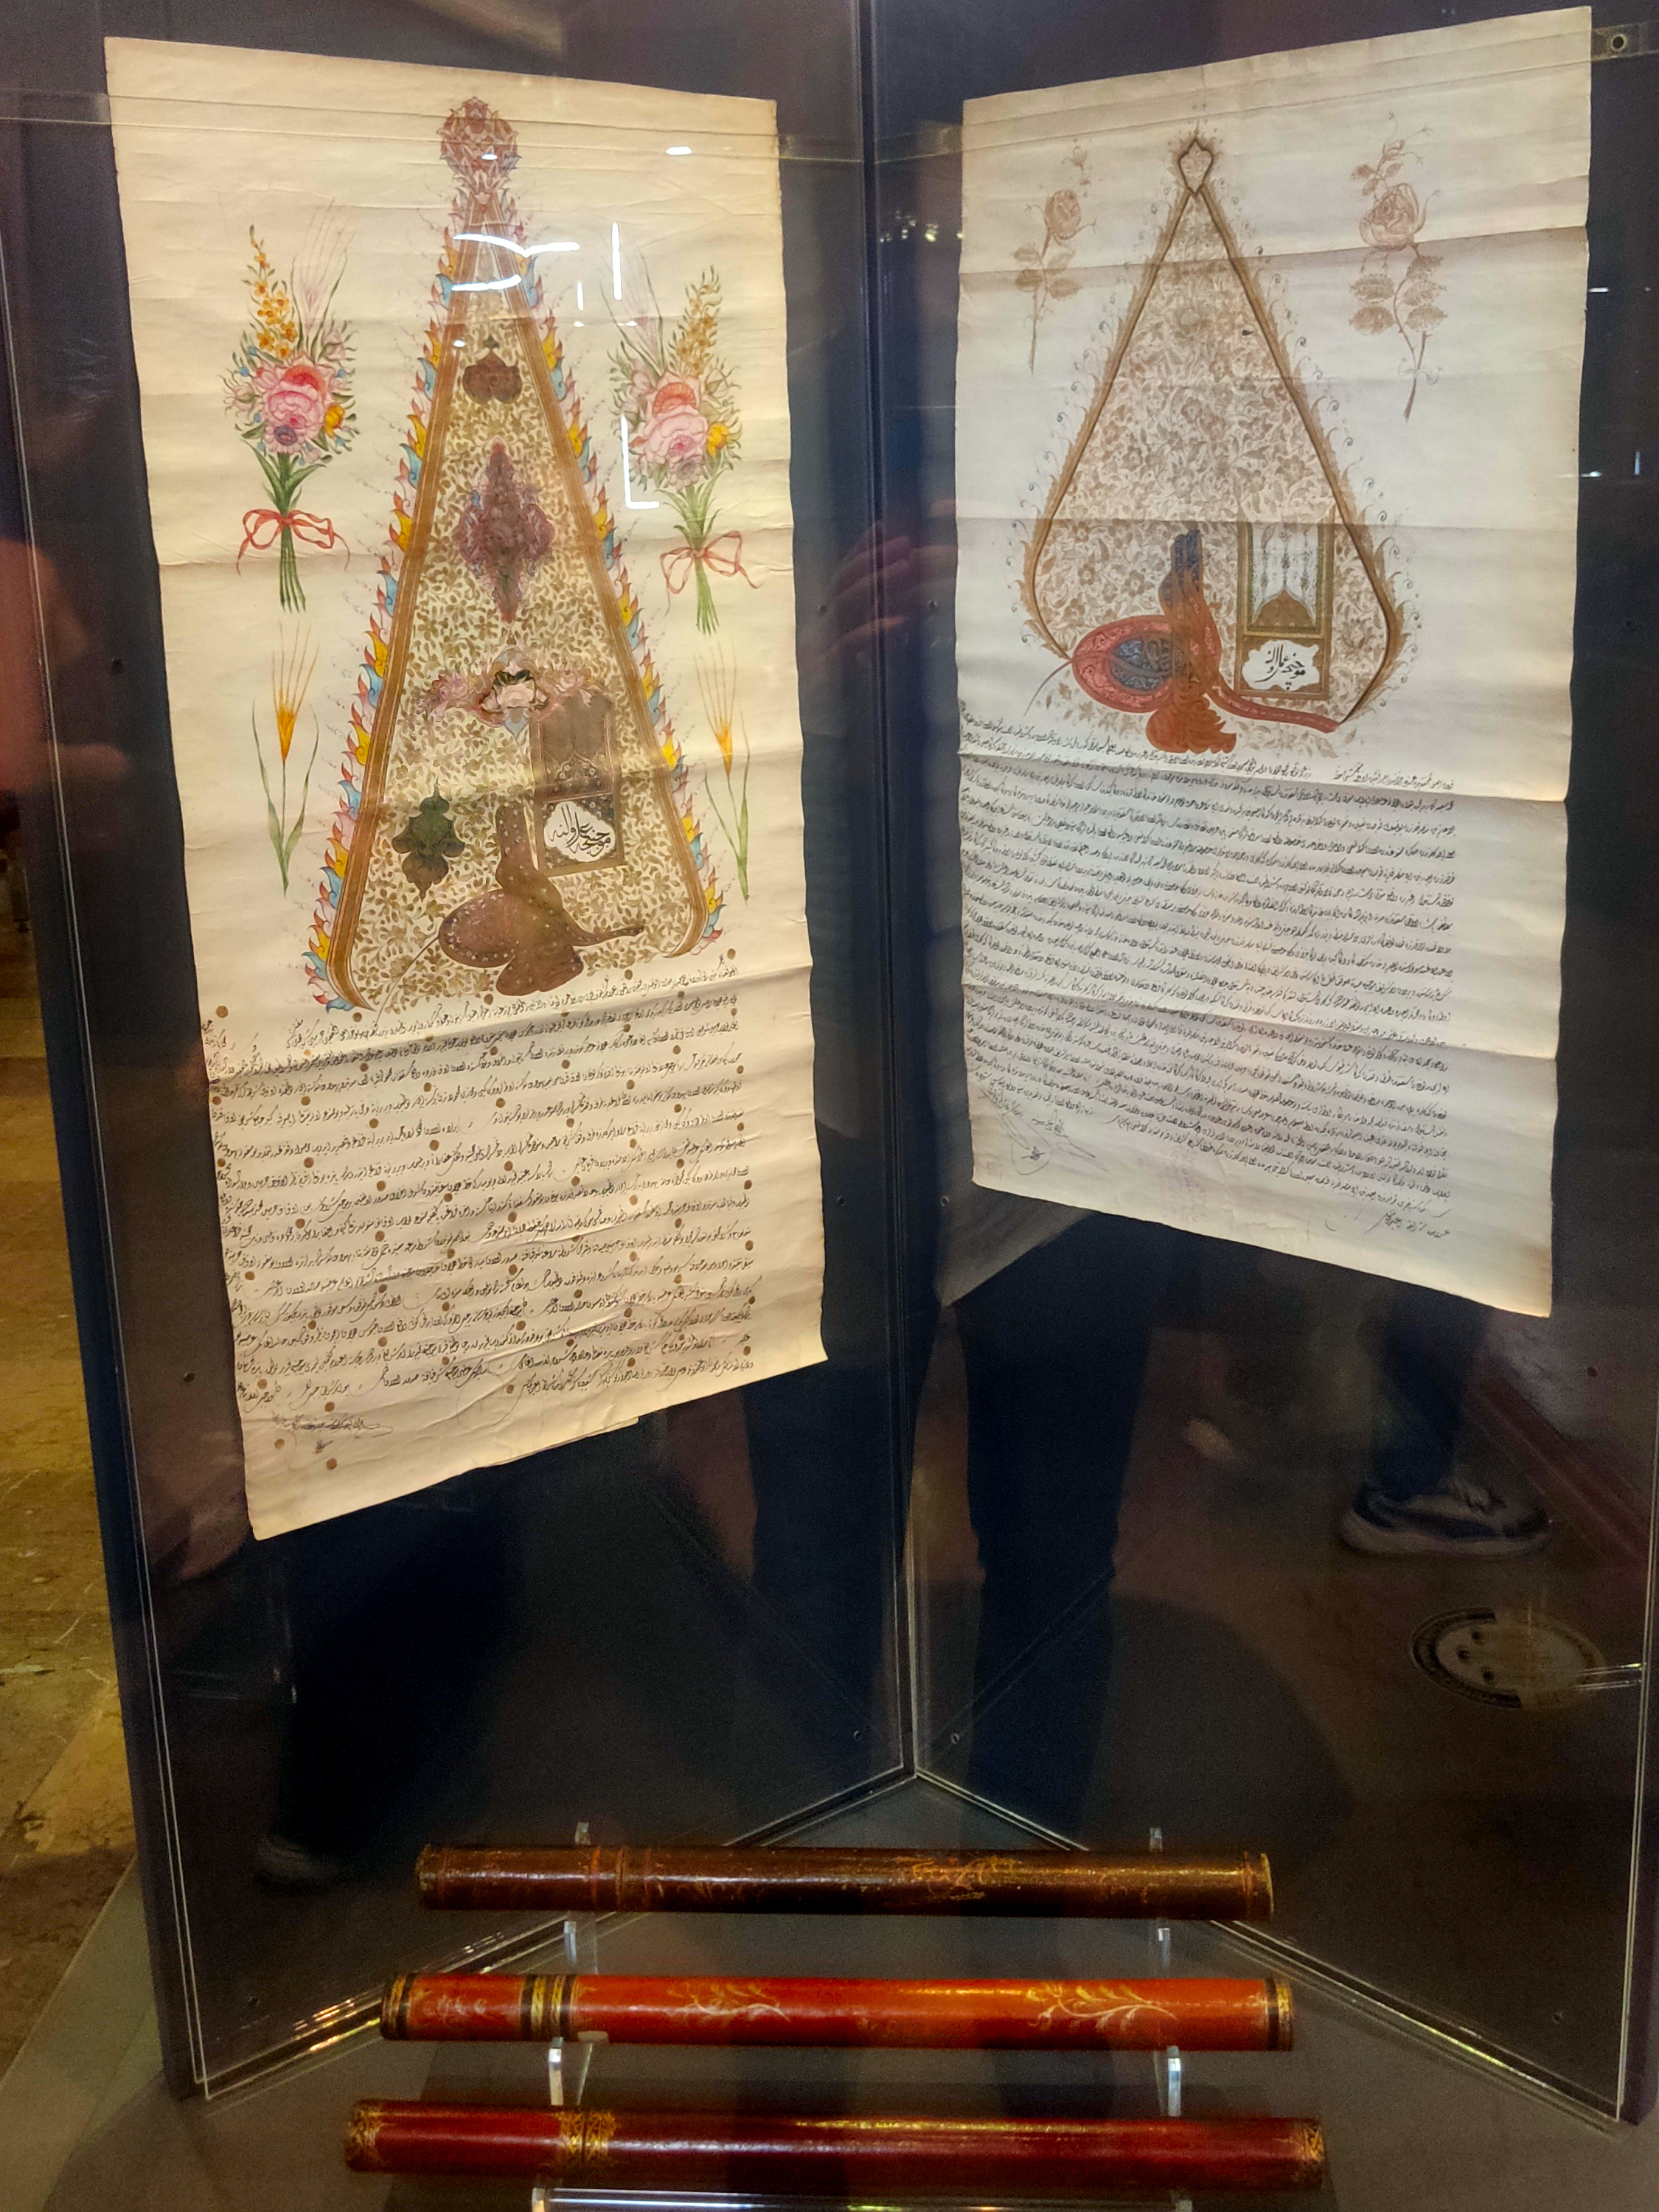
\includegraphics[height=0.25\textheight]{assets/kubur.jpg}
    }
    \hspace{10pt}
    \subfigure[Zübdetü't Tevârîh]{
        \includegraphics[height=0.25\textheight]{assets/zubdetut_tevarih.jpg}
    }
    \caption{El Yazması Eserler}
\end{figure}
\indent Bu eserlere ek olarak, Osmanlı hanedanına ait mücheveler ve takılar da bu salonda incelenebilir. Bunlar arasında Hürrem Sultan'ın takıları öne çıkan eserlerden biridir. Hanedan ailesi tarafından kullanılmış altın ve yakut işlemeli kemerler bu kısımda sergilenmektedir.
\begin{figure}[H]
    \centering
    \subfigure[Takılar]{
        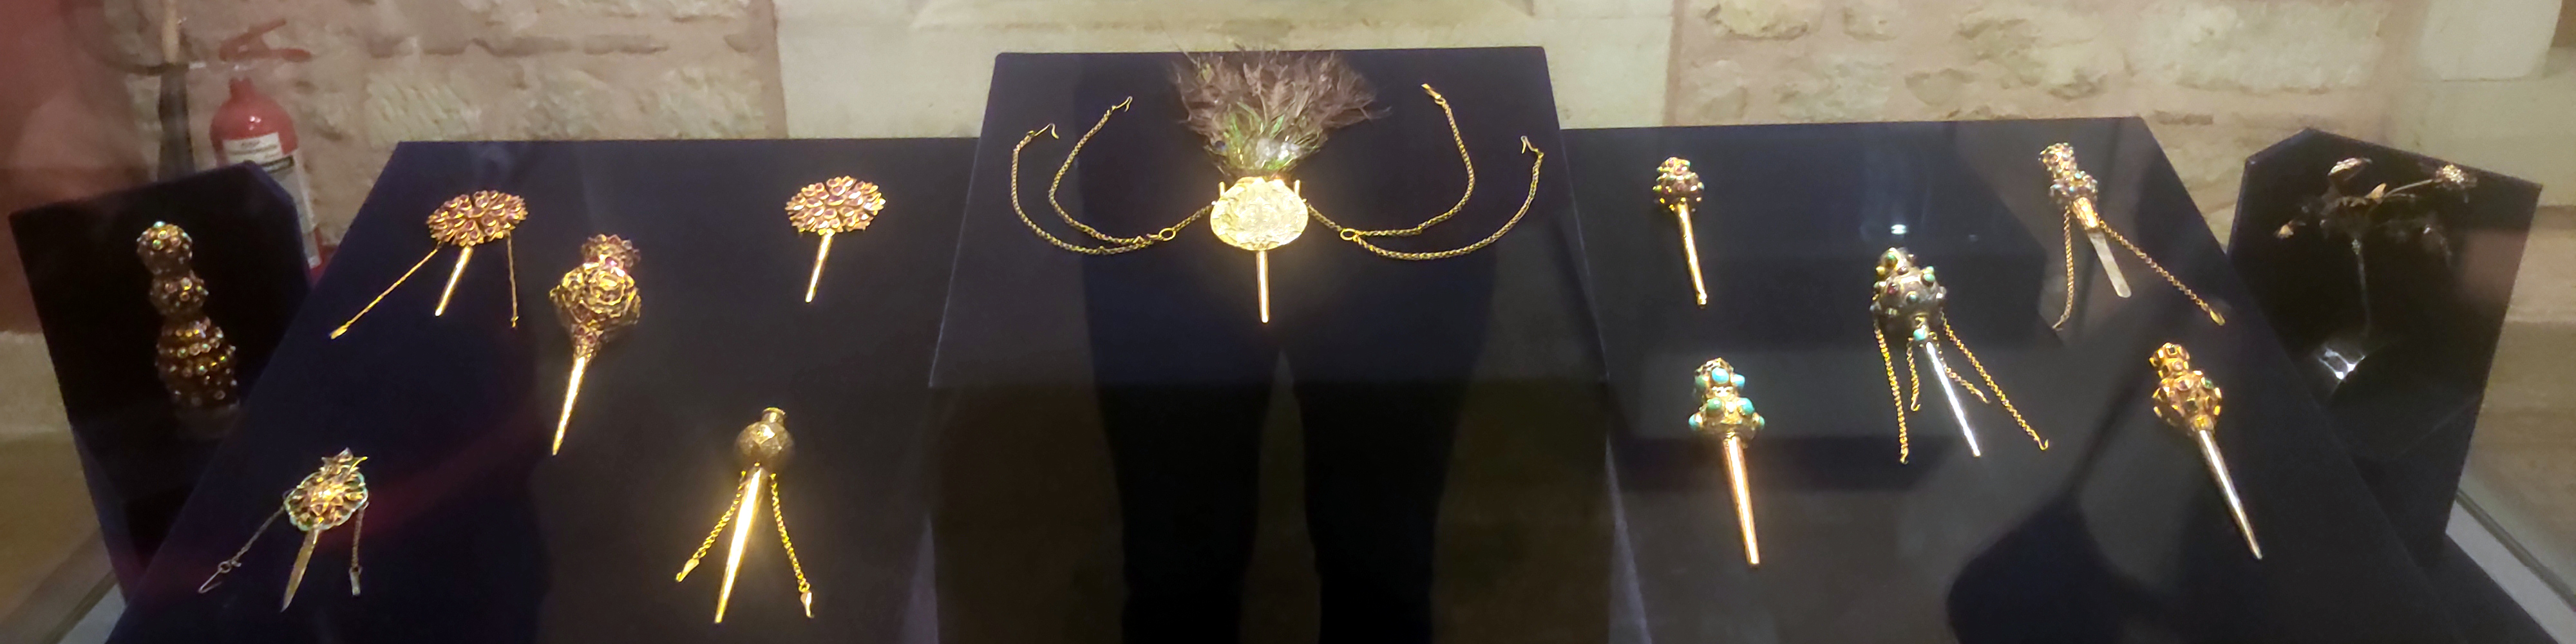
\includegraphics[width=0.9\linewidth]{assets/jewelry.jpg}
        \label{fig:jewelry}
    }
    \hfill
    \subfigure[Mücheverler ve Takılar]{
        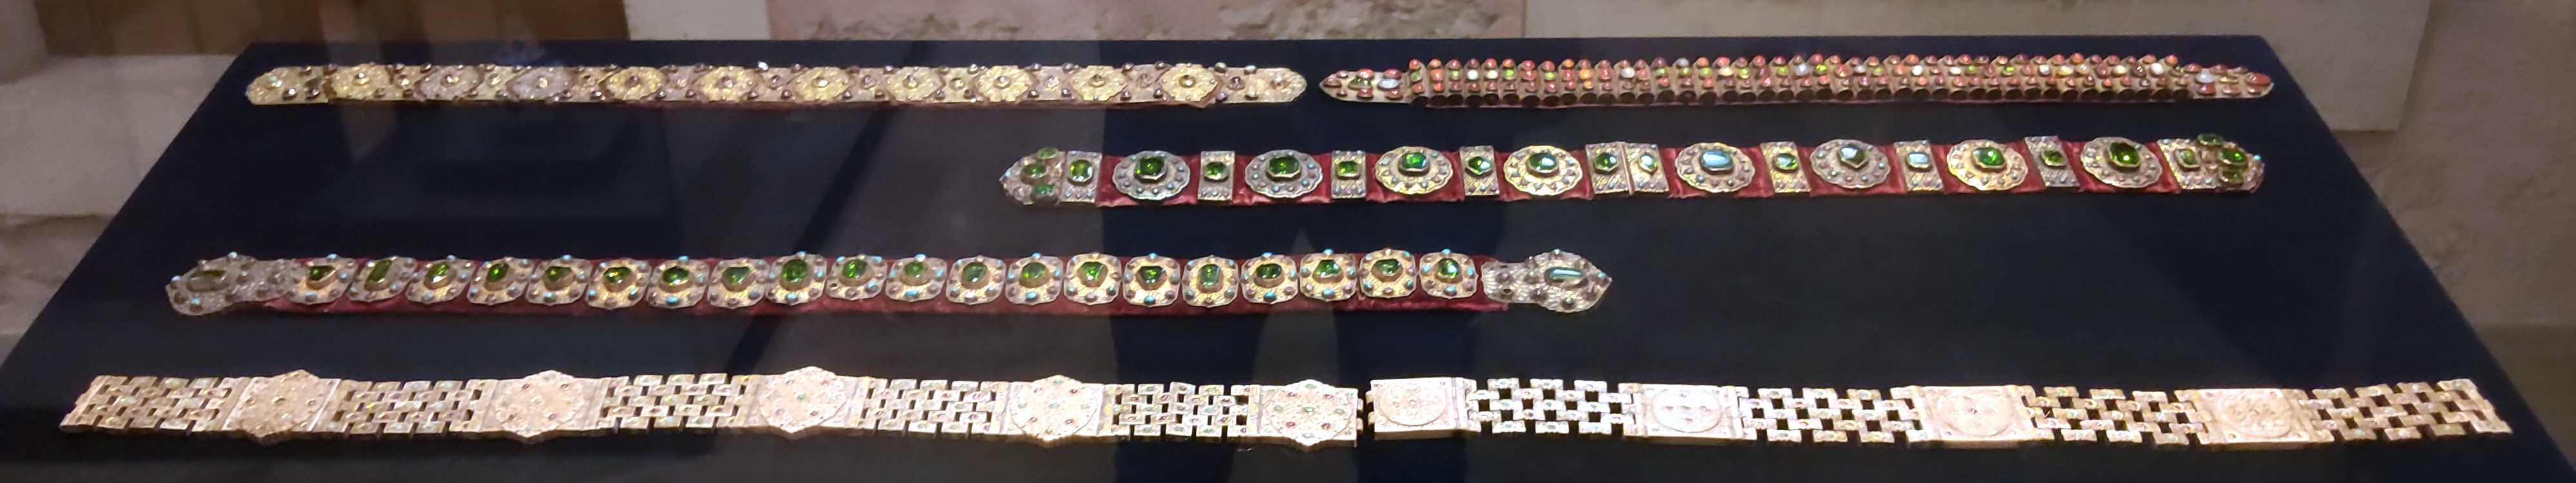
\includegraphics[width=0.9\linewidth]{assets/belts.jpg}
        \label{fig:belts}
    }
    \caption{Hanedan Takıları ve Kemerleri}
\end{figure}
\subsection{Etnografya Salonu}
\indent\indent Osmanlı eserlerinin sergilendiği salonun hemen altında kalan kısımda müzenin etnografya salonu bulunmaktadır. Etnografya, antropolojinin bira dalı olup sistematik bir şekilde kültürleri incelemektedir. Adından da anlaşılacağı gibi bu salonda ağırlıklı olarak Osmanlı toplumunun günlük yaşam kültürü sergilenmektedir. Salonun girişinde Osmanlı Devleti'nin kısa bir kronolojisi bulunmaktadır. Bu kronolojiyi geçince, II. Abdülhamid'in kaleska tarzı arabalarından bir tanesi karşımıza çıkmaktadır. Buranın hemen yanında Osmanlı toplumunun günlük yaşamında önemli yer tutan iki önemli kültüre ait eşyalar sergilnemektedir. Bunların ilki hamam kültürüdür. Osmanlı hamamlarında sıkça kullanılan hamam kurnası, terlik, peştemal, ponza taşı gibi eşyalar burada incelenebilir. Buradaki terliklerde göze çarpan özellik ise topuk büyüklükleridir. Eğer terliğin topukları büyük ise, kirli suyun olduğu yerde giyilmesi uygundur. Küçük topuklular ise temiz suyun olduğu yerlerde tercih edilmektedir. Hamam sergisinin karşısında kahve kültürüne ait sergi bulunmaktadır. Burada da ge. Osmanlı dönemine ait kahve değirmenleri, kahve kavurucuları ve soğutucuları, cezveler ve fincanlar incelenebilir. Bu alandaki bri başka sergi ise hattatların kullandığı hokka, divit ve kalemlerdir. Bunların yanı sıra 19. yüzyıl mobilyaları ve kadın giyisileri de yine etnografya salonunda sergilenmektedir.\newline
\indent Bu kısımda en ilgi çekici eser ise, \textit{İstanbul'un Manzara-i Umûmiyesi} isimli resmin halıya nakşedilmiş haliydi. Bu resmin orijinali, II. Abdülhamid dönemi halk ressamı Mehmet Hulusi tarafından yapılmıştır. Resmin yapılış amacı, İstanbul'daki yapıları rakamlarla anlatmaktı. Müzedeki halı ise sadece manzara resmedilmiş şekilde sergilenmektedir. (Şekil \ref{fig:istanbul_view})\newline
\begin{figure}[H]
    \centering
    \includegraphics[height=0.4\textheight,width=0.9\linewidth]{assets/istanbul_view.jpg}
    \caption{İstanbul'un Manzara-i Umûmiyesi}
    \label{fig:istanbul_view}
\end{figure}
\indent \textit{İstanbul'un Manzara-i Umûmiyesi} adlı eserin altında Haliç'i ve İstanbul Boğazı'nı kapatan zincirin bir parçası sergilenmektedir. Zincir uygulaması, Bizans döneminde Haliç'i savaş gemilerine kapatmak için kullanılan bir uygulamaydı. Osmanlılar da İstanbul'un fethinden sonra, Sarayburnu ile Haliç arasını bu zincirle kapatarak, Kız Kulesi'nde kurulan daire ile gümrük vergisi toplama uygulamasını bir süre uygulamışlardır. Ticarete gelen gemiler Kız Kulesi'ne yanaşarak gerekli işlemleri tamamladıktan sonra Haliç'e giriş yapmaktaydı. Bir deprem sonrası Kız Kulesi'nin zarar görmesinden dolayı bu uygulama 17. yüzyılda kalkmıştır.
\section{Dördüncü Hafta - Türk İslam Eserleri Müzesi}
\indent\indent Müzenin uzmanlarından Tarık Akar tarafından, müzenin arka bahçesindeki Azize Euphemia Kilisesi kalıntıları gezildi ve İbrahim Paşa Sarayı bölümleri ve müzenin arka bahçesi hakkında bilgi verildi.
\subsection{Azize Euphemia Kilisesi}
\indent\indent Azize Euphemia, MS 307 yılında Ares için düzenlenen şenliklere katılmayı reddettiği için Khalkedon'da(bugün Kadıköy) tutuklanmıştır. Ölüm tarihini ise kaynaklar 16 Eylül 307 olarak bildirmektedir. Daha sonra Hıristiyanlıkta şehit olarak kabul edilecek Euhemia'nın bedeni bütün olarak bir tabutun içinde muhafaza edildi. Tam olarak ne zaman yapıldığı bilimese de 4.yüzyılın sonlarına doğru Khalkedon'da, Euphemia adına yapılmış bir kilisenin varlığı bilinmektedir. 451 yılında Khalkedon konsili, bu kilisede toplanmıştır. 7.yüzyılın başındaki Pers akınları ile hasar gören kiliseden Euphemia'nın \textit{bozulmamış bedeni} buradan alınıp, Konstantinopolis surları içine getirilmiştir. Daha sonra Hippodrom'un bitişiğindeki Antiokhos sarayının yanına Euphemia adına yeni bir kilise inşa edildi. Bu kilise, Hippodrom'daki Azize Euhemia Kilisesi olarak anılmıştır.\cite{euphemia}\newline
\indent 1951-52 yıllarında, Adalet Sarayı'nın yapımı için ifa edilen kazılarda ortaya çıkan kiliseden günümüze sadece silüeti kalmıştır. Yerdeki kalıntılarda bir apsis göze çarpıyor. Apsisin karşısında kalan ve tahminen girişin yer aldığı duvar kısmen ayaktadır. Bu duvar üzerindeki freskolar da yine kısmen görülebilmektedir.
\begin{figure}[H]
    \centering
    \subfigure[Fresko - 1]{
        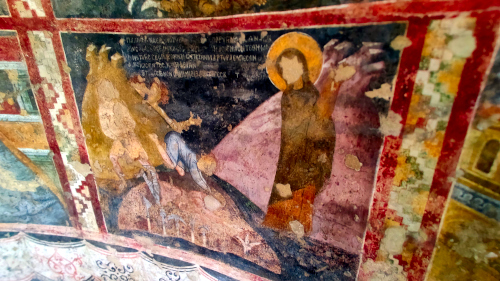
\includegraphics[height=0.15\textheight]{assets/euphemia_fresco_1.jpg}
    }
    \subfigure[Fresko - 2]{
        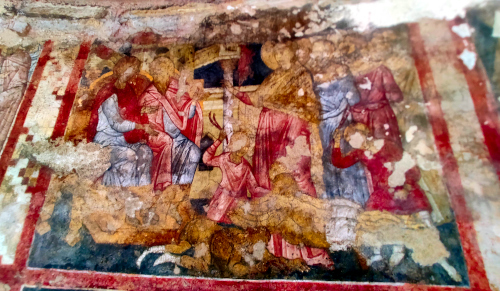
\includegraphics[height=0.15\textheight]{assets/euphemia_fresco_2.jpg}
    }
    \subfigure[Duvar]{
        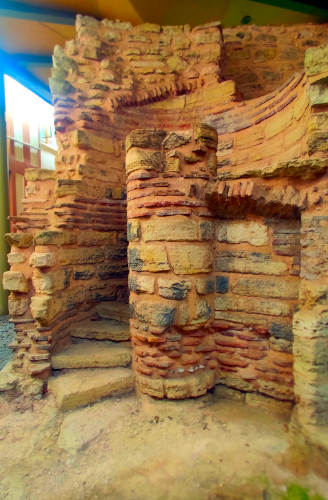
\includegraphics[height=0.15\textheight]{assets/euphemia_wall.jpg}
    }
    \subfigure[Apsis]{
        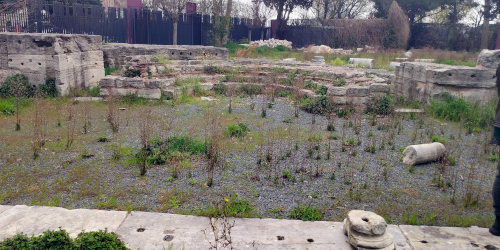
\includegraphics[height=0.2\textheight]{assets/euphemia_apsis.jpg}
    }
    \caption{Azize Euphemia Kilisesi Kalıntıları}
\end{figure}
\subsection{Pargalı İbrahim Paşa Sarayı İç Avlusu}
\indent\indent Oldukça geniş bir alan üzerine inla edilmiş olan İbrahim Paşa Sarayı'nın gümüzde sadece 2/5 ayaktadır. Dört avlu, ahırlar, bir kule ve hazine binasından oluşan saray, oldukça geniş bir araziye yayılmış durumdaydı. Sarayın üçüncü avlusuna 1910 yılında Mimar Vedat Tek'in projelendirdiği Defter-i Hakani(Tapu Kadastro Müdürlüğü)(günümüzde Ayasofya Müzesi) binası yapılmıştır. Sarayın bir diğer avlusu ise 1939 yılında Adliye Sarayı'nın inşası için yıkılmıştır. 1970lerde restorasyon geçiren sarayın ikinci avlusu, 1983 yılında Türk İslâm Eserleri Müzesi'ne tahsis edilmiştir. Saraya gelen misafirleri karşılamak için kullanılan müze avlusunun batı duvarının arkasında ise, İbrahim Paşa'nın kendi hususi avlusu bulunmaktadır. Dikdörtgen forma sahip bu avludan, iki katlı şekilde inşa edilmiş şekilde sarayın ikametgâh kısmı bulunmaktadır.
\section{Beşinci Hafta - Pera Müzesi}
\subsection{Müzeye Genel Bakış}
\indent\indent 1883 yılında \textit{Orient Express}(Doğu Ekspresi)'nin hizmete sunulmasıyla, Pera bölgesinde Avrupa tarzı otelcilik hizmetleri oluşmaya başladı. Dönemin İstanbul'unda han tarzı konaklama servisleri, Doğu Ekspresi'nin lüksüne ayak uyduracak seviyede değillerdi. Bu sebeple, bugünkü Meşrutiyet Caddesi üzerinde 1892 yılında Büyük Londra Oteli ve Pera Palace, 1893 yılında da Bristol Otel inşa edildi. Büyük Londra Oteli ve Pera Palace günümüzde de hizmet vermeye devam ederken, Bristol Otel 1980'de kapanıyor ve bina \textit{Esbank}(Eskişehir Bankası) tarafından satın alınıyor. Esbank'ın 2001 yılında kapanmasıyla birlikte, Suna ve İnan Kıraç Vakfı binayı 2003 yılında satın alıyor. Bina, 2003-2005 yılları arasında restoratör mimar Sinan Genim'in hazırladığı proje doğrultusunda restore edildi. Bu restorasyon ile cadde kotunun 8 metre aşağısına inilereke iki kat bodrum ilavesiyle bina 8 kata ulaştı.\newline
\indent En üst kattan aşağı doğru gezilecek şekilde tasarlanan müzenin en üst 3 katı, her yıl müze küratörleri tarafından 3-4 farklı sergiye ev sahipliği yapıyor. Ziyaretin yapıldığı tarihte en üst iki kat Kanadalı sanatçı Marcel Dzama'nın \textit{Dancing with the Moon}(Ay Işığyla Dans) isimli sergisine ayrılmıştı. Üçüncü katta ise, müzenin kuruluşunda büyük katkıları bulunan ve 2007 yılında vefat eden Samih Rıfat'a vefa sergisi bulunmaktaydı. Müzenin ikinci ve birinci katları ise Kıraç ailesinin koleksiyonlarına ayrılmıştır. İkinci katta ailenin resim koleksiyonu, birinci katta ise ağırlık ve Kütahya çinileri koleksiyonları sergilenmektedir. 
\subsection{Marcel Dzama Sergisi}
\indent\indent Marcel Dzama, şu anda New York'ta yaşayan 1974 Winnipeg doğumlu Kanadalı sanatçıdır. Çok yönlü bir sanatçı olan Dzama, ağırlık olarak resim, heykel, kağıt katlama, kısa film gibi alanlarda eserler üretmektedir.\newline
\indent Hayattaki deneyimlerinden beslenen Dzama'nın eserlerinde hayvan figürleri ön plana çıkıyor. Çocukluğunda dedesinin çiftliğinde ayı, geyik, yarasa, kokarca gibi hayvanları çok sık görmesinin etkisi olduğunu söylüyor. Bu hayvanlardan yarasalarla daha belirgin bir anısı var. İlkokulunda konteyner sınıflarda öğrenim gören Dzama, bir gün bu konteynerların fileyle sarılmış kısmını kesmeye heveslenir. Fileyi kesmesiyle beraber onlarca yarası kaçışır ve bu sahne Dzama üzerinde derin etki yaratır.\newline
\indent Bir diğer sık rastlanan motif ise ay. Çocukluğundan beri aya karşı bir ilgisi olduğunu belirten yazar, Meksika ve özellikle Fas'a yaptığı gezilerden sonra ay motifini daha çok kullandığını ekliyor. \textit{Blue Moon of Morroco} isminde bir sergisi ve \textit{To Live On The Moon(For Lorca)} isimli İspanyol şair Federico Garcia Lorca'ya ithaf ettiği kısa müzikal filmi bulunmaktadır.\newline
\indent Protest tarafını da resimlerinde sık sık ön plana çıkarmaktadır. Dünyadaki diktatörlüklere ve kötü yönetimlere karşı olan duruşunu sık sık vurguluyor. Eserlerinde Trump, Putin, Stalin gibi liderlere karikatürize edilmiş şekillerde rastlıyoruz. George Orwell'in 1984 romanına yaptığı göndermeler yine diktatörlük eleştirisi olarak göze çarpıyor.\newline
\indent Bir diğer eleştiri odağı ise patriarka. Eserlerinde kadınların daha ön plana çıkması gerektiğini, devrimin ve barışın kadınların ellerinden geleceğini ifade etmektedir. Özellikle \textit{The revolution will be female}(Devrim dişi olacak) ve \textit{Let the Women rule after the clown is through}(Palyaço gittikten sonra kadınlar yönetsin) isimli eserlerinde bu mesajlar daha açık görülmektedir.\newline
\begin{figure}[H]
    \centering
    \subfigure[The revolution will be female]{
        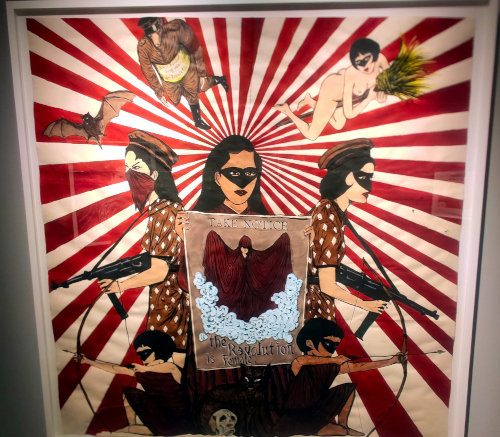
\includegraphics[width=0.45\linewidth]{assets/dzama_2.jpg}
    }
    \hfill
    \subfigure[Let the Women rule after the clown is through]{
        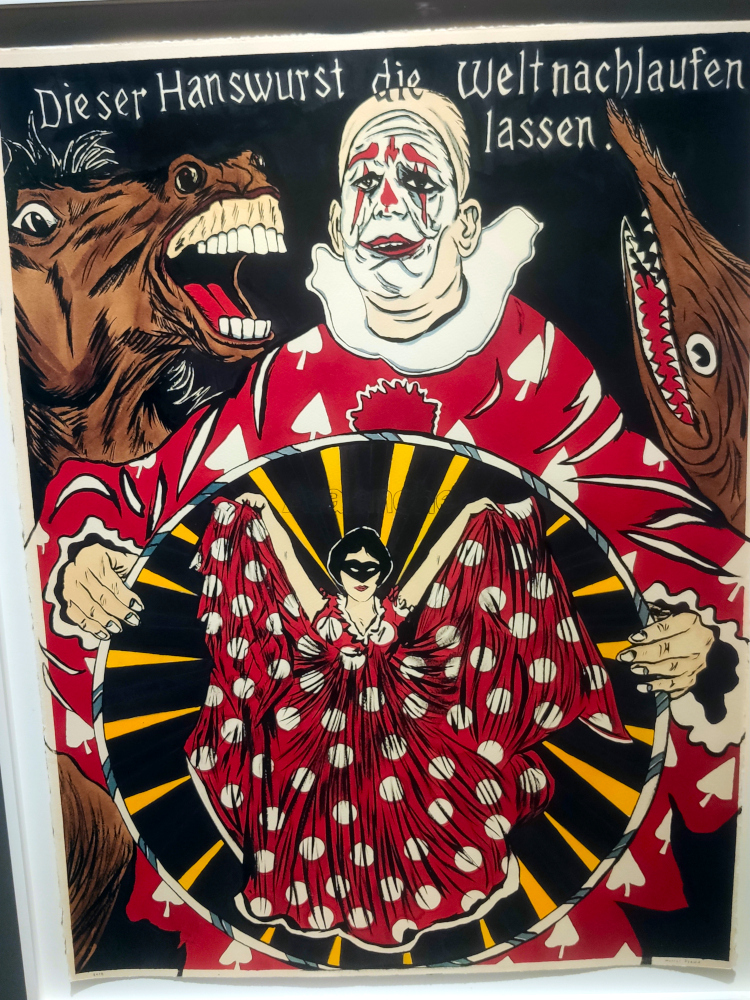
\includegraphics[width=0.30\linewidth]{assets/dzama_3.jpg}
    }
    \caption{Marcel Dzama'nın Protest Eserleri}
\end{figure}
\indent Joseph Beuys, Marcel Duchamp va dadaizm etkilerine eserlerinde sık sık rastlıyoruz. Kelime oyunlarını seven Dzama, \textit{Be little Beuys and Dada might buy you a Bauhaus} isimli eserindr \textit{boys} kelimesini \textit{Beuys} ve \textit{daddy} kelimesini \textit{dada} şeklinde yazarak Joseph Beuys ve dadaizme gönderme yapmaktadır. Öte yandan Marcel Duchamp'ın(kendisi iyi bir satranç oyuncusudur) satrançı eserlerinde kullanmaya başlamasından etkilenmiş; satranç ile savaş arasında ilgi kurarak heykellerinde ve kısa filmlerinde bu temayı işlemiştir.
\begin{figure}[H]
    \centering
    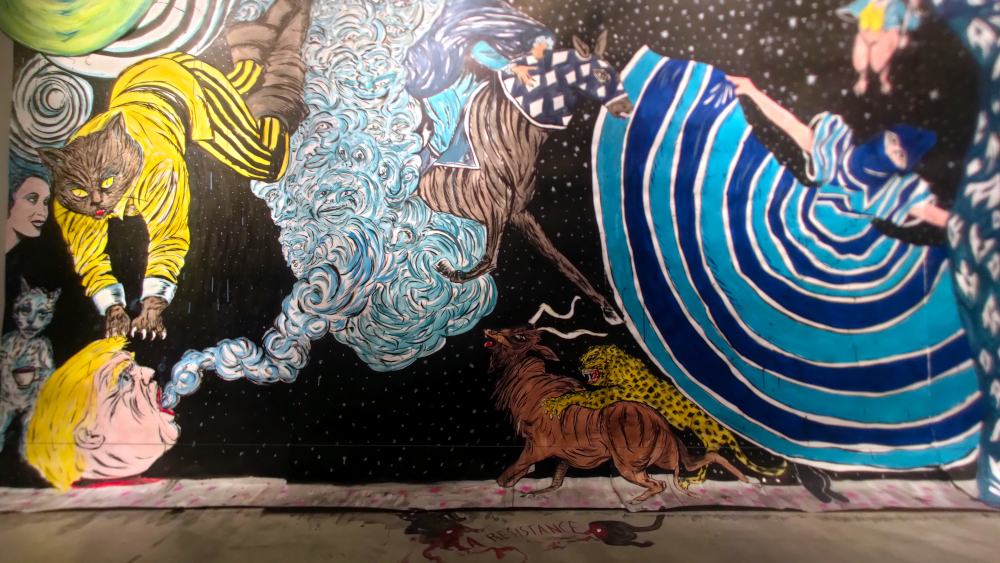
\includegraphics[width=0.9\linewidth]{assets/dzama_1.jpg}
    \caption{Be little Beuys and Dada might buy you a Bauhaus}
\end{figure}
\subsection{Samih Rifat Sergisi}
\begin{wrapfigure}{r}{0.3\textwidth}
    \centering
    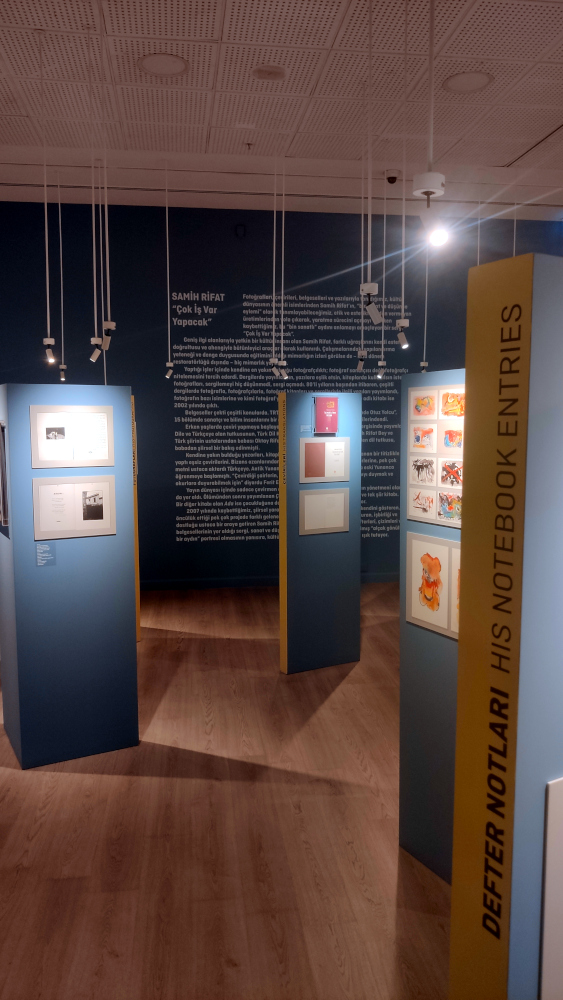
\includegraphics[width=0.25\textwidth]{assets/samih_rifat.jpg}
    \caption{Samih Rifat Sergisi}
\end{wrapfigure}
\indent\indent Samih Rifat, 24 Kasım 1945 tarihinde İstanbul'da doğmuştur. Ünlü şair Oktay Rifat'ın oğludur. İlköğrenimini Beylerbeyi İlkokulu’nda, ortaöğrenimini Saint Benoît Fransız Lisesi’nde tamamlamıştır. Yükseköğrenimini İstanbul Teknik Üniversitesi (İTÜ) Mimarlık Fakültesi’nde tamamlayan Rifat, bir süre kamu kurumlarında mimar olarak görev yapmıştır.\newline
\indent Meslek hayatının ilerleyen dönemlerinde belgesel ve reklam filmi yönetmenliğine yönelmiş; aynı zamanda fotoğrafçılık alanında da üretimlerde bulunmuştur. Üniversite yıllarında başladığı çeviri çalışmalarını 1980’li yıllarda Yazko Çeviri dergisinde yayımlayarak sürdürmüştür. René Char, Jacques Prévert, André Verdet, Jean Follain, Paul Valéry, Vladimir Mayakovski, Konstantinos Kavafis, Amin Maalouf, Yorgos Seferis ve Le Corbusier gibi önemli şair ve yazarlardan Türkçeye çeviriler yapmıştır. Bunlarla beraber, \textit{Aries} ve \textit{Fol} isimlerinde iki dergi yayımlamıştır.\newline
\indent Fotoğrafçılıkla da yakından ilgilenen Samih Rifat, 1980’li yıllardan itibaren çeşitli dergilerde yayımlanan yazılarına kendi fotoğraflarıyla eşlik etmiştir. Bunun yanı sıra, belgesel filmler çekmiş ve müzikle de ilgilenmiştir. Klasik gitar çalan Rifat, 1981 yılında İstanbul Filarmoni Derneği’nin düzenlediği ilk İstanbul Uluslararası Gitar Festivali'nin organizasyonunda görev almış ve festival kapsamında sanatçı Mutlu Torun ile birlikte sahne almıştır.\newline
\indent Müzenin üçüncü katında, 4 Ağustos 2007 tarihinde aramızdan ayrılan Samih Rifat için bir nevi vefa sergisi bulunmaktadır. Sergide Samih Rifat'ın çevirileri, yazıları, yayımladığı dergileri, besteleri, çizimleri ve fotoğraf eserleri bulunmaktadır.
\subsection{Oryantalist Resim ve Ağırlık Koleksiyonu}
\indent\indent Müzenin ikinci katında, 17. yüzyıldan 20. yüzyıl başlarına uzanan bir dönemi kapsayan eserler sergilenmektedir. Bu koleksiyonda, Avrupalı ressamların Osmanlı dünyasını ve Türkiye coğrafyasını betimleyen yapıtlarının yanı sıra, Osmanlı sanatçılarının bu dönemdeki karşılıklı etkileşimleri yansıtan eserlerine de yer verilmektedir. İmparatorluğun son iki yüzyılına dair geniş bir görsel panorama sunan bu bölümde, Osman Hamdi Bey’in eserleri ile ünlü \textit{Kaplumbağa Terbiyecisi} adlı tablosu da bulunmaktadır.\newline
\indent \textit{Elçi Alayı}, dört adet tablodan oluşan ve Flaman asıllı Fransız ressamı Jean Baptiste Vanmour tarafından resmedilmiş eserdir. Vanmour, 1699 yılında İstanbul’a Fransız elçi Ferriol ile birlikte gelmiş ve Osmanlı toplumuna dair detaylı figüratif betimlemeler yapmıştır. İlk tabloda elçi alayının Galata sırtlarından Haliç'e inişi resmedilmiştir. Elçi Alayı'nın geçtiği yer, günümüzde Pera Müzesi'nin önündeki Meşrutiyet Caddesi'dir. İkinci tabloda ise alayın Topkapı Sarayı'na teşrifi anlatılmıştır. Tablodan kabulün ulufe divanı ile birşeştirlmiş bir elçi divanında, yani büyük divanda yapıldığını anlamaktayız. Alayın Bab-ı Hümayun'dan giriş yaptığı sırada, elçi heyetini etkilemek için yapılan Çanak Yağması ikinici tablodaki ilginç detaylardan biridir. Üçüncü tabloda ise, heyet şerefine Kubbealtı'nda verilen yemek bulunmaktır. Burada, Kasr-ı Adl adlı kafeste III.Ahmed'in gölgesini görmekteyiz. Dördünce tabloda ise, heyetin padişah III.Ahmed tarafından kabulu anlatılmıştır. \newline
\indent Buradaki en eski eser ise, Kutsal Roma İmparatoru II. Ferdinand tarafından Osmanlı İmparatoru 4. Murad'a elçi olarak gönderilen Hans Ludwig von Kuefstein’in elçilik heyetinde olan Avusturyalı ressamlar Franz Hermann, Hans Gemminger ve Hermann'ın yardımcısı olduğu anlaşılan Valentin Mueller tarafından yapılan 1654 tarihli \textit{Türk Hareminden Bir Sahne} isimli bir tablodur. Ters perspektif şeklinde resmedilmiş olan eserde, ön kısımdaki kompozisyon haremde misafir karşılama ve dans teması işlenmiştir. Arkadakı kompozisyonda da haremin bir odası tasvir edilmiştir. Resmi yapan kişilerin haremi görme şansı olmadığından, tablo büyük bir ihtimalle harem hakkında duyduklarının ve öğrendiklerinin yansımasıdır. Resimdeki halı motiflerinin daha İran tarzı olması belki de bundandır.\newline
\indent Koleksiyondaki en değerli eser aynı zamanda bir Türk tarafından yapılmış en pahalı tablo olup, 2003 yılında bir müzayedede 3.5milyon dolara alınmış olan Osman Hamdi Bey'in \textit{Kaplumbağa Terbiyecisi} isimli tablosudur. Osman Hamdi Bey, Paris'teki eğitimi sırasında resim dersleri almış ve batı resmini oryantal öğelerle harmanlayarak Türkiye resim sanatında yeni bir dönem başlatmıştır. Müzenin bu kısmında Kaplumbağa Terbiyecisi ile birlikte dört tane daha eseri sergilenmektedir.\newline
\indent Tablonun resimlediği sahnede yerdeki yeşillikleri yemekte olan kaplumbağaları düşünceli bir tavırla izleyen Doğulu giysiler içinde bir Osman Hamdi Bey'in otoportresini görürüz.  Elinde bir ney tutmakta, sırtında nakkare veya kudüm cinsinden bir vurmalı çalgı durmaktadır. Önünde durduğu pencerenin üstünde yer alan sivri kemerli alınlıkta \textit{Şifa’al-kulûp lika’al Mahbub} yani \textit{Kalplerin şifası, Sevgiliyle (Hz. Muhammed) buluşmaktır} yazılıdır. Mekân olarak, sanatçının resimlerinde sıkça karşımıza çıkan Bursa Yeşil Cami’nin hünkar mahfili kullanılmıştır. Adamın elinde, sırtında yer alan çalgılar derviş olabileceğini akla getirse de, başlığı Elbise-i Osmaniye’de yemeniler dolanmış keçe kalpak olarak tanımlanan \textit{Mardinli Kürd} tipinin başlığına benzer. Eser, Türkiye'nin tembel ve umursamaz bürokrasisine bir eleştiri niteliğindedir. Kaplumbağalar, yavaş ve içine kapanık bir hayvan olduğu için bürokrasinin tembelliğini ve tepkisizliğini simgelemektedir. Eserin merkezinde adam ise kaplumbağaları müzik(sanat) ile eğitmeyi denemektedir. Bezgin bir halde resmedilmiş adamın yüzünden muvaffak olamadığını anlıyoruz. Kaplumbağa Terbiyecisi, Osman Hamdi Bey’in koleksiyondaki beş eserinden biridir.\newline
\indent Müzenin ilk katı, prehistorik çağlardan günümüze Anadolu coğrafyasında gündelik hayatın tanıklığını yapmış objelere ev sahipliği yapıyor. Koleksiyon prehistorik dönem, Klasik Dönem, Beylikler ve Osmanlı Dönemi ile Erken Cumhuriyet dönemi başta olmak üzere Anadolu’nun ev sahipliği yaptığı birçok uygarlığa ait materyal bulunmaktadır. Arazi ölçümünden her türlü alışverişe, mimarlıktan kuyumculuğa, denizcilikten eczacılığa, astronomiden zaman ölçüm aletlerine kadar farklı alanlardan birçok ağırlık, uzunluk, hacim ölçüsünü bünyesinde barındıran bu koleksiyon Anadolu’nun zengin ve çok çeşitli kültürüne tarihsel bir perspektif sunmaktadır.
\begin{figure}[H]
    \centering
    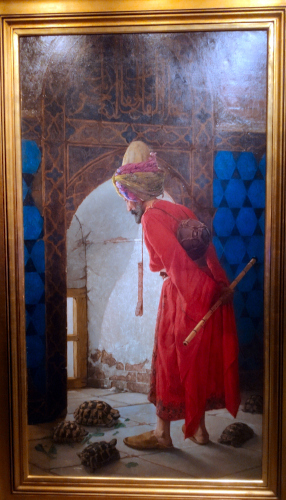
\includegraphics[height=0.95\textheight]{assets/kaplumbaga_terbiyecisi.jpg}
    \caption{Osman Hamdi Bey'in Kaplumbağa Terbiyecisi Tablosu}
\end{figure}
\section{Altıncı Hafta\\İslam Bilim ve Teknoloji Tarihi Müzesi}
\subsection{Fuat Sezgin}
\indent\indent İstanbul İslam Bilim ve Teknoloji Tarihi Müzesi, Fuat Sezgin'in öncülüğünde 25 Mayıs 2008 tarihinde hizmete girmiştir. 23 Ekim 1924'te doğan Fuat Sezgin, İstanbul Üniversitesi Edebiyat Fakültesi Şarkiyat Enstitüsü'nde öğrenim gördü. 1950 yılında Arap Dili ve Edebiyatı bölümünde \textit{Buhari'nin Kaynakları} adlı doktora tezini yayımladı. 27 Mayıs 1960 asker darbesinin ertesinde, askeri darbe yönetiminin üniversitelerden ihraç ettiği ve 147'ler olarak anılan akademisyenler arasındaydı. İhraç sonrası 1961 yılında Almanya'ya giden Fuat Sezgin, Frankfurt'taki Johann Wolfgnag Goethe Üniversitesi'nde misafir doçent olarak dersler vermeye başladı. 1965 yılında da profesör unvanını aldı.\newline
\indent İstanbul'dayken başladığı 7.-14.yüzyıllar arası Arap-İslam edeibyat tarihi üzerine yaptığı çalışmalarının ilk cildini 1967 yılında, son cildini ise 2000 yılında yayımlamıştır. 13 cild şeklinde yayımladığı \textit{Geschichte des arabischen Schrifttums} isimli eser, Arap-İslam kültürünün coğrafya, haritacılık, edebiyat tarihine ışık tutmaktadır.
\subsection{İstanbul İslam Bilim ve Teknoloji Tarihi Müzesi}
\indent\indent İstanbul İslam Bilim ve Teknoloji Tarihi Müzesi, iki kattan müteşekkil olup; astronomi, zaman ve saatler, savaş aletleri, madenler, matematik ve geometri, mimari ve şehircilik, kimya, optik gibi çeşitli sergiler ihtiva etmektedir. Aşağıda, daha öne çıkan astronomi, zaman ve saat ve savaş aletleri sergilerine değineceğiz.
\subsubsection{Astronomi Sergisi}
\indent\indent Ağırlıklı olarak sekstantların va gözlemevlerinin minyatürlerinin sergilnediği kısımıdır. Sekstant, yerküre üzerinde bulunulan yerin enlemini ve boylamını belirlemek amacıyla, bir gök cismiyle ufuk düzlemi arasındaki açısal mesafeyi ölçmekte kullanılan optik seyir cihazı.\cite{sekstant} 60 derecelik yaya sahip olduğu için Latincedeki sextus(altıda bir, altıncı) kelimesinden hareketle sextant adı verilmiştir. Sekstantla açı ölçmek için, gemici sekstant dürbününden, ufuk hattına bakar. Gemici, gemi güvertesinde dik olarak durduğu ve gemiyle beraber sallandığı için ölçülecek açı hiç değişmez. Güneşin aynalardan yansıyan görüntüsü tam ufuk hattıyla çakıştığı an sekstant açısı okunur.\newline
\indent Bu kısımda, 903 yılında doğmuş Abdurrahman es-Sufî'nin tasavvur ettiği gök kürenin de bir örneği incelenebilir. Abdurrahman es-Sûfî, sabit yıldızların sistematik incelenmesi ve kataloglanmasında Batlamyus’tan sonra en önemli isimlerden biridir. Kitâbü Ṣuveri’l-kevâkibi’s̱-s̱âbite adlı eserinde kırk sekiz yıldız takımını ayrıntılı biçimde ele alarak yıldızların konum, parlaklık ve renk bilgilerini açıklamış, Batlamyus’un terminolojisini Arapçaya kazandırmıştır. Es-Sûfî’nin tanımladığı terimlerden doksan dördü modern astronomi literatüründe hâlen kullanılmaktadır.\cite{dia_8}\newline
\begin{figure}[H]
    \centering
    \subfigure[Sekstantlar]{
        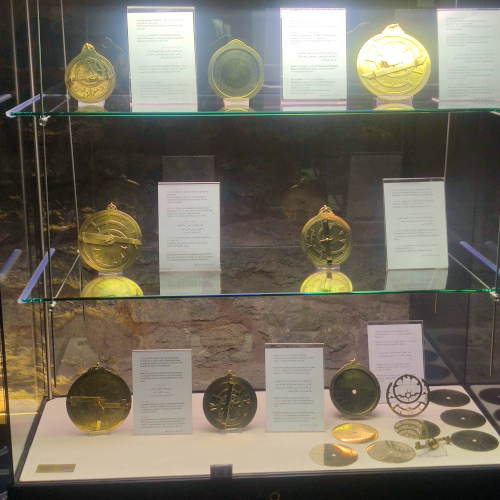
\includegraphics[width=0.55\textwidth,height=0.45\textheight]{assets/sekstant.jpg}
    }
    \hfill
    \subfigure[Abdurrahman es-Sufî'nin Gök Küresi]{
        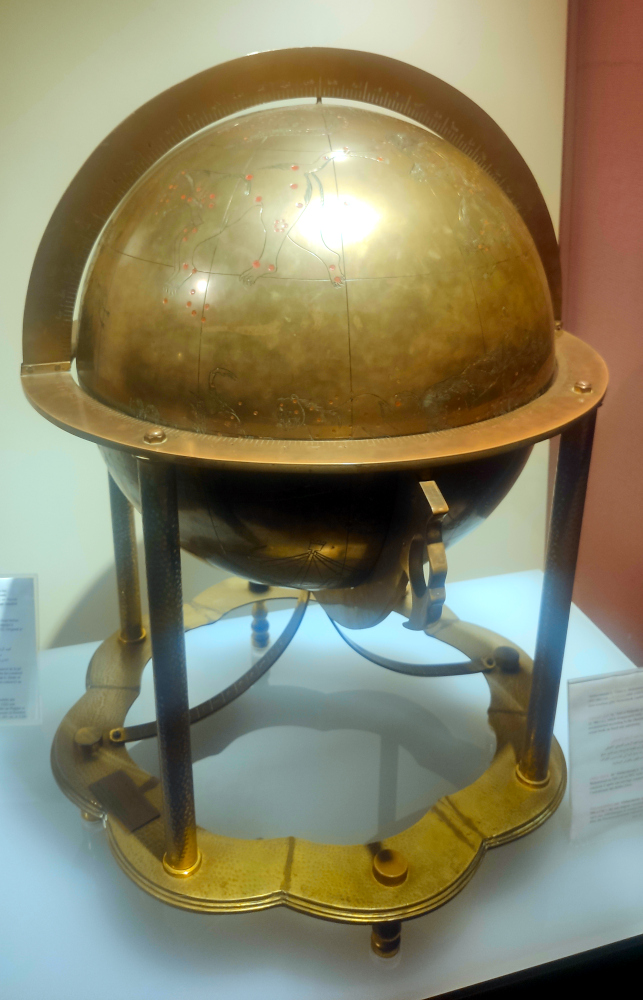
\includegraphics[width=0.4\textwidth,height=0.45\textheight]{assets/sphere.jpg}
    }
    \caption{Astronomi ile ilgili eserler}
\end{figure}
\subsection{Zaman ve Saat}
\indent\indent Bu bölümde, Arap ve İslam bilim insanlarının zamanı ölçmek için ürettiği saatlerin prototiplerini incelemek mümkün. Müzenin en dikkat çekici eserlerinde birisi de Fas Ḳaraviyyīn Camii’nde bulunan su saati modelidir. Bu model, günü 24 saate bölen, günümüze ulaşmış en eski su saatidir. Her saatin 4er dakikaya(yani 15 bölüme) bölümlendiği bir saat kadranında tasarlanmıştır. Her dört dakikada küçük bir küre, her bir saatte ise büyük bir küre 24 pirinç kaseden birisine düşer ve bir ses oluşturur. 24 saat zarfında toplam 360 küçük ve 24 büyük küre kaselere, oradan da bir toplama haznesine düşer. Akustik sinyallere ilaveten, her saat başı, geçen zamana dair genel bir bakış veren ve uzaktan da görülebilen ahşap kapılardan birisi kapanır. Düzenek, dökülen su aracılığıyla harekete geçirilir. Bu su, ipli makaralar vasıtasıyla işleyen bütün kısımların bağlantıda olduğu bir şamandrayı aşağı indirir. Düzenli akış, tam olarak basınç ayarlayan bir cihaz vasıtasıyla sağlanır.\newline
\begin{figure}[H]
    \centering
    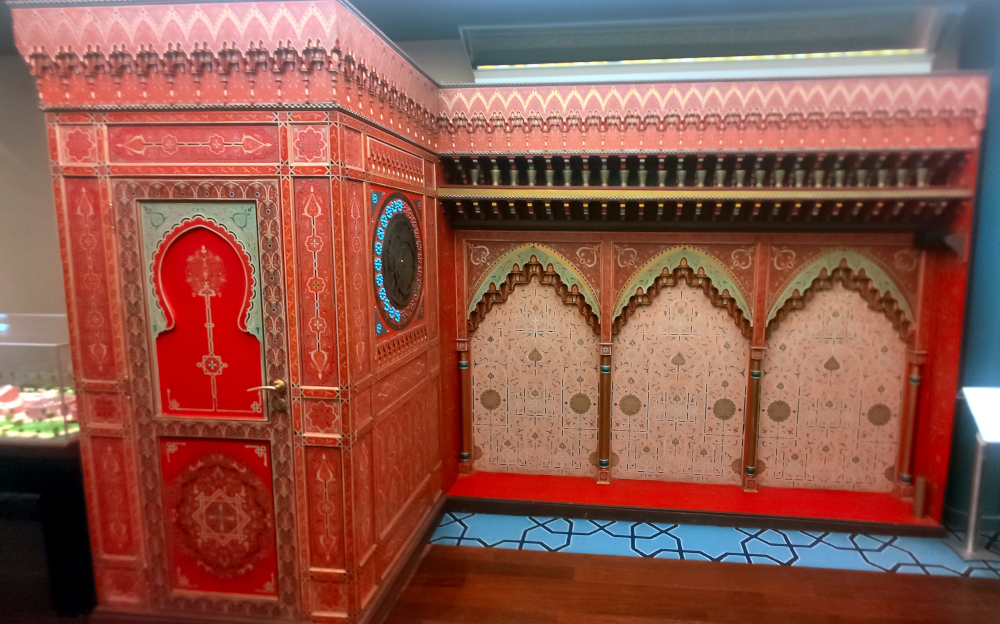
\includegraphics[width=0.95\linewidth]{assets/water_clock.jpg}
    \caption{Fas Su Saati}
\end{figure}
\newpage
\subsection{Savaş Aletleri}
\begin{wrapfigure}{r}{0.2\textwidth}
    \centering
    \includegraphics[width=0.2\textwidth]{assets/lageri.jpg}
    \caption{Lagari Hasan Çelebi'nin Roketi}
\end{wrapfigure}
\indent\indent Türk ve İslam devletlerinin yaptığı savaşlarda kullanılan aletlerin sergilendiği bölüm. Ağırlıklı olarak kuşatma aletlerini ve mancınık modellerini ihtiva etmektedir. Bu kısımda en ilgi çekici eser ise, Lagari Hasan Çelebi'nin tasarladığı roket modelidir. Lagari Hasan Çelebi, 1632 ya da 1633 yılında Sarayburnu'nda IV.Murad'ın da hazır bulunduğu denemede, kendisini tasarladığı rokete bağlatmış olduğu halde roketi ateşletmiştir. 300 metre kadar yükseldikten sonra barutu biten roket serbest düşüşe geçmiş, Lagari Hasan Çelebi kollarına bağladığı kanatları açarak yumuşak iniş yapmıştır. Hikayenin doğruluğu oldukca şüphelidir, çünkü Lagari Hasan Çelebi'yi anlatan tek kaynak Evliya Çelebi'nin \textit{Seyahatname} isimle eseridir.\newline

\newpage
\printbibliography

\end{document}
